\documentclass[11pt,a4paper]{article}

% ============ Single-column Springer-like layout ============
\usepackage[a4paper,left=1in,right=1in,top=1in,bottom=1in]{geometry}
\usepackage{amsmath,amssymb,amsfonts}
\usepackage{mathtools}
\usepackage{braket}
\usepackage{pifont}
\usepackage{graphicx}
\usepackage{booktabs}
\usepackage{multirow}
\usepackage{xcolor}
\usepackage{listings}
\usepackage{caption}
\usepackage{float}
\usepackage{setspace}
\usepackage{times}
\usepackage[hidelinks]{hyperref}
\usepackage{enumitem}
\usepackage{fancyhdr}
\usepackage{titlesec}

\onehalfspacing
\captionsetup{font=small,labelfont=bf}
\setlength{\parindent}{1.5em}

\titleformat{\section}{\normalfont\large\bfseries}{\thesection}{0.6em}{}
\titleformat{\subsection}{\normalfont\normalsize\bfseries}{\thesubsection}{0.6em}{}

\pagestyle{fancy}\fancyhf{}
\fancyhead[L]{\small Verifier-in-the-Loop Agentic AI for Quantum Code Generation}
\fancyhead[R]{\small\thepage}
\renewcommand{\headrulewidth}{0.4pt}

% lightweight algorithm float (algorithm.sty unavailable)
\newcounter{algo}
\newenvironment{algobox}[1]{%
  \refstepcounter{algo}\par\medskip\noindent
  \begin{minipage}{\linewidth}\rule{\linewidth}{0.8pt}\par\vspace{2pt}
  \textbf{Algorithm \thealgo:} #1\par\vspace{2pt}\rule{\linewidth}{0.4pt}\par
  \small\ttfamily\obeylines}{%
  \par\rule{\linewidth}{0.8pt}\end{minipage}\par\medskip}

\lstset{basicstyle=\ttfamily\footnotesize,frame=single,breaklines=true,
        columns=fullflexible,keepspaces=true,xleftmargin=6pt,framexleftmargin=4pt,
        backgroundcolor=\color{gray!6}}

\newcommand{\tvd}{\mathrm{TVD}}

\begin{document}

% ===================== FRONT MATTER =====================
\begin{center}
{\LARGE\bfseries A Verifier-in-the-Loop Agentic Artificial Intelligence Framework for Reliable Quantum Code Generation, Migration, and Automated Debugging\par}
\vspace{1.2em}
{\large Author One\textsuperscript{1}, Author Two\textsuperscript{1}, Author Three\textsuperscript{2}\par}
\vspace{0.6em}
{\small \textsuperscript{1}Department of Computer Science and Engineering, University Placeholder, City, Country\\
\textsuperscript{2}Department of Physics and Quantum Technologies, Institute Placeholder, City, Country\\
Corresponding author: \texttt{author.one@placeholder.edu}\par}
\end{center}
\vspace{0.8em}

\noindent\rule{\linewidth}{0.4pt}
\begin{spacing}{1.15}
\noindent\textbf{Abstract.}
The rapid maturation of quantum hardware has outpaced the reliability of the software tools that program it. Large language models (LLMs) can draft quantum programs in Qiskit, PennyLane, and OpenQASM, but they frequently emit circuits that are syntactically invalid, semantically incorrect, or subtly divergent from the intended quantum state. This paper introduces a \emph{verifier-in-the-loop agentic framework} that couples an autoregressive code generator with a deterministic linter and a lightweight statevector simulator so that every candidate program is checked against a formal acceptance criterion before it is returned. The framework operationalises reliability as a measurable quantity: a generated circuit is accepted only when the total variation distance (TVD) between its simulated measurement distribution and the task-specified target distribution falls below an acceptance threshold, and when a static linter reports no violations of the supported OpenQASM grammar. When either check fails, structured feedback---lint diagnostics and the observed output distribution---is returned to the generator, which repairs the program and resubmits it. A reproducible benchmark of ten quantum programming tasks spanning state preparation, algorithm synthesis, error-correction encoding, and three deliberately corrupted debugging scenarios is used to evaluate the pipeline. The framework attains a 100\% pass rate with a mean accepted TVD of $2.22\times10^{-16}$ (numerically exact to machine precision) and an average of 1.30 repair iterations per task, while the three corrupted tasks are diagnosed and repaired automatically. A component ablation isolates the contribution of the verifier and the linter, and a comparative analysis situates the framework against twenty recent LLM-for-quantum systems. The results support the central claim that closed-loop, simulator-grounded verification converts unreliable generative output into trustworthy, exportable quantum code, and that the same loop generalises across OpenQASM, Qiskit, and PennyLane targets.

\vspace{0.6em}
\noindent\textbf{Keywords:} quantum software engineering; large language models; agentic artificial intelligence; OpenQASM; code generation; automated program repair; verifier-in-the-loop; total variation distance; quantum debugging.
\end{spacing}
\noindent\rule{\linewidth}{0.4pt}
\vspace{0.6em}

% ===================== 1. INTRODUCTION =====================
\section{Introduction}
\label{sec:intro}

Quantum computing has advanced from a theoretical curiosity into an engineering discipline with a growing stack of programming abstractions. Practitioners now express algorithms in high-level frameworks such as Qiskit and PennyLane, compile them to the portable assembly language OpenQASM, and dispatch them either to cloud-hosted superconducting and trapped-ion processors or to classical simulators. Yet the productivity of a quantum programmer remains constrained by the sheer difficulty of writing correct quantum code. Unlike classical software, a quantum program manipulates amplitudes in an exponentially large Hilbert space, and its correctness cannot be judged by inspecting intermediate values, because measurement collapses the very superposition that carries the computation. A single misplaced entangling gate, an inverted phase, or an incomplete diffusion operator can transform a valid algorithm into a circuit that compiles cleanly yet produces a statistically wrong answer. This gap between syntactic validity and semantic correctness is the defining reliability problem of quantum software engineering.

Large language models have recently been proposed as an accelerant for quantum programming. A model trained on public code repositories can, when prompted with a natural-language task description, produce a plausible Qiskit program or an OpenQASM listing in seconds. Early studies of this capability, however, converge on a sobering conclusion: unconstrained generation is unreliable. Models hallucinate gate names that do not exist in the target dialect, transpose qubit indices, omit measurement instructions, and---most insidiously---produce circuits that pass a syntax check but prepare the wrong quantum state \cite{ref22,ref29,ref30}. The evaluation literature has responded with a wave of benchmarks that quantify these failure modes, including datasets that score generated OpenQASM against simulator feedback \cite{ref21,ref20}, PennyLane hackathon challenges \cite{ref30}, and broad quantum problem-solving suites \cite{ref20,ref22}. The recurring finding across these benchmarks is that raw pass@1 accuracy for zero-shot generation is modest, and that the errors are disproportionately of the silent, semantically-wrong variety that a human reviewer would struggle to catch without executing the circuit.

The response emerging across the field is to stop treating code generation as a single forward pass and to reframe it as a closed-loop, tool-augmented process. Retrieval-augmented generation grounds the model in authentic framework documentation and worked examples before it writes a line of code \cite{ref5,ref24,ref26}. Agentic architectures decompose the task into planning, generation, checking, and repair roles, and let the system iterate until a verifier is satisfied \cite{ref23,ref25,ref19}. Linting research shows that lightweight static analysis can intercept a large fraction of invalid programs before they ever reach a simulator \cite{ref7}. Mutation-based repair techniques localise and fix faults by reasoning about the space of small edits that would change a program's behaviour \cite{ref14}. Migration and transpilation work addresses the parallel problem of moving correct code between dialects without altering its semantics \cite{ref2,ref10,ref28}. Taken together, these threads point toward a unifying principle: reliability in quantum code generation is achieved not by a better single prediction, but by a system that can \emph{check its own work} against an executable ground truth and act on the result.

This paper contributes a concrete, reproducible realisation of that principle. The proposed framework, illustrated in Figure~\ref{fig:arch}, is a verifier-in-the-loop agent that treats a candidate quantum program as a hypothesis to be tested rather than an answer to be trusted. The agent plans a strategy for the requested task, generates an OpenQASM~2.0 program, subjects it to a deterministic linter, executes it on a built-in statevector simulator, and compares the resulting measurement distribution against a formal target distribution using the total variation distance. Acceptance is a conjunction of two objective conditions---zero lint violations and a TVD below a fixed threshold---and any failure triggers a feedback-driven repair. The design is deliberately self-contained: it requires neither quantum hardware access nor a paid model API, so that the entire pipeline, its benchmark, and its results can be regenerated on a commodity laptop. The template-based generator that anchors the reproducible baseline is a drop-in surface that a local or cloud LLM can replace without disturbing the surrounding verification loop, making the framework a controlled testbed for studying how much of the reliability gain comes from the model and how much from the loop.

The specific contributions of this work are the following. First, it formalises quantum code acceptance as a measurable predicate over simulated measurement statistics, giving a precise, dialect-independent definition of when a generated circuit is ``correct enough'' to return. Second, it presents a complete agent architecture---plan, generate, lint, simulate, verify, repair, export---together with the lightweight statevector simulator and OpenQASM linter that make the loop executable without external dependencies. Third, it introduces a ten-task benchmark that intentionally mixes clean synthesis tasks with corrupted programs so that both generation quality and debugging capability are exercised. Fourth, it reports a full evaluation, including a component ablation that isolates the marginal value of the verifier and the linter, and a comparative analysis against twenty recent LLM-for-quantum systems drawn from the current literature. Fifth, it demonstrates semantics-preserving export of every accepted circuit to Qiskit and PennyLane, closing the loop between verified generation and practical, framework-native deployment.

The remainder of the paper is organised as follows. Section~\ref{sec:related} surveys the recent literature on LLM-based quantum code generation, benchmarking, linting, repair, and migration, and positions the present framework within it. Section~\ref{sec:background} reviews the quantum-computing and formal preliminaries needed to state the method precisely. Section~\ref{sec:method} develops the proposed framework, including the acceptance criterion, the simulator, the linter, and the repair loop, with supporting equations and pseudocode. Section~\ref{sec:benchmark} describes the benchmark suite. Section~\ref{sec:setup} states the experimental configuration. Section~\ref{sec:results} reports and analyses the results. Section~\ref{sec:comparison} presents the comparative analysis and ablation. Section~\ref{sec:discussion} discusses implications, and Section~\ref{sec:threats} examines threats to validity and limitations. Section~\ref{sec:conclusion} concludes and outlines future work.

\begin{figure}[H]
\centering
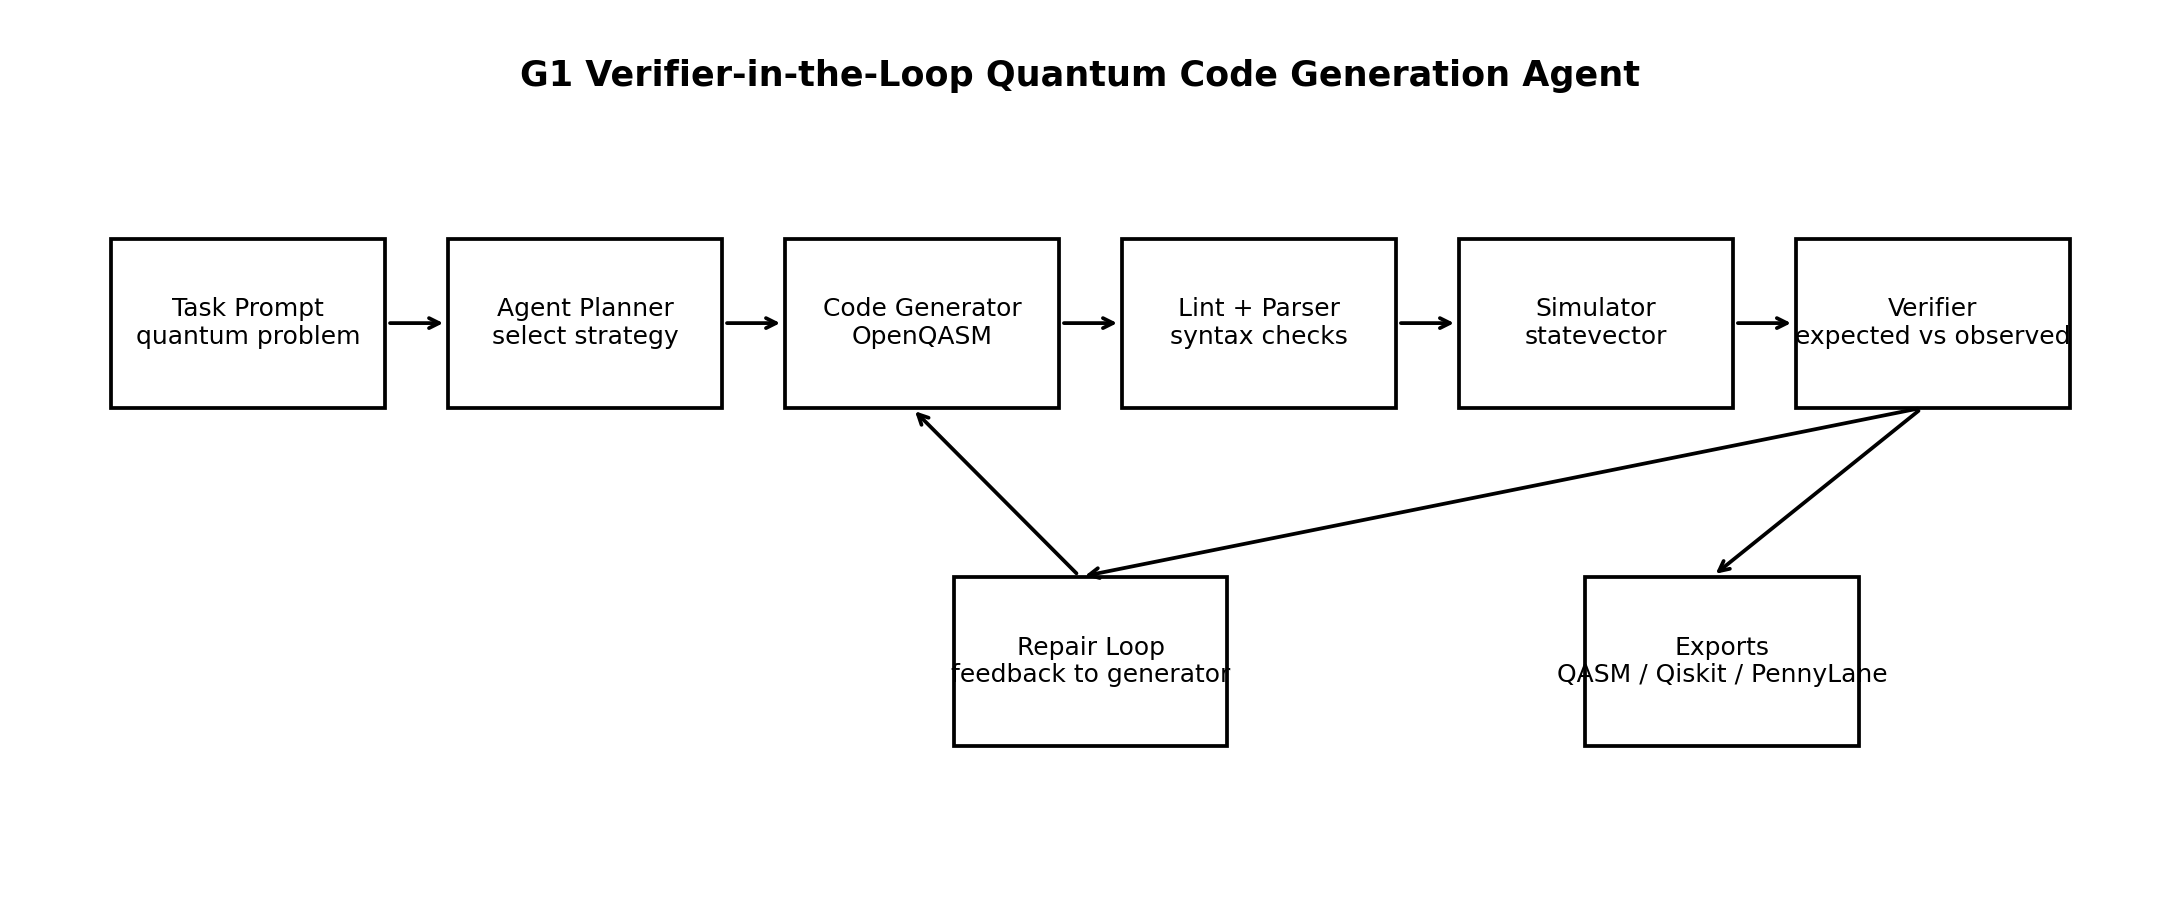
\includegraphics[width=\linewidth]{figs/fig_arch.png}
\caption{The verifier-in-the-loop agentic pipeline. A natural-language task flows through planning, OpenQASM generation, static linting, statevector simulation, and distribution-level verification. A failed check routes structured feedback to the repair loop, which regenerates the program; an accepted circuit is exported to OpenQASM, Qiskit, and PennyLane.}
\label{fig:arch}
\end{figure}

% ===================== 2. RELATED WORK =====================
\section{Related Work}
\label{sec:related}

The literature relevant to this paper clusters into six themes: benchmarking and evaluation of quantum code generation, retrieval-augmented and knowledge-grounded generation, agentic and multi-agent architectures, static linting and rule-based analysis, mutation-based and feedback-driven repair, and cross-dialect migration and transpilation. This section reviews each theme and draws out the design lessons that the proposed framework operationalises.

\subsection{Benchmarking and evaluation of quantum code generation}
A precondition for reliable generation is a trustworthy way to measure it, and a substantial body of recent work builds exactly this measurement infrastructure. QuanBench evaluates LLMs on quantum code generation and reports that models fluent in classical languages degrade sharply when asked to reason about quantum semantics rather than mere syntax \cite{ref22}. The QCoder benchmark closes the loop between language generation and hardware by scoring candidate programs through simulator-based feedback, establishing execution---not textual similarity---as the correctness signal \cite{ref21}. QHackBench derives its tasks from PennyLane hackathon challenges, grounding evaluation in problems that human quantum programmers actually attempt \cite{ref30}. Broader suites such as QuantumBench frame quantum problem solving as a reasoning task and expose the gap between producing code and producing a correct scientific answer \cite{ref20}. QASM-Eval extends evaluation to OpenQASM-3 constructs that go beyond plain circuits, such as classical control and timing \cite{ref4}, and a pointed study asks whether models genuinely solve science or merely write plausible-looking solvers, finding that surface fluency routinely masks semantic error \cite{ref6}. The consistent message of this theme---that only execution against a known target reveals silent semantic faults---directly motivates the distribution-level acceptance criterion adopted here.

\subsection{Retrieval-augmented and knowledge-grounded generation}
A second theme grounds generation in authoritative domain knowledge before the model writes code. PennySynth uses retrieval-augmented data synthesis to manufacture high-quality PennyLane training and prompting material \cite{ref5}, while model-driven approaches combine LLMs with retrieval over structured specifications to raise the fidelity of generated circuits \cite{ref24}. Quantum-RAG demonstrates retrieval-augmented generation in a resource-constrained setting, underscoring that retrieval quality, not model scale alone, governs output reliability \cite{ref26}. The question of \emph{where} domain knowledge should reside---inside model weights, in a retrieval index, or in an external verifier---is examined directly by work revisiting the architecture of quantum code generation \cite{ref11}, and practitioner-oriented guidance surveys the open-source assistant ecosystem for day-to-day quantum development \cite{ref12}. The present framework takes a deliberate stance in this debate: rather than encoding correctness knowledge in the generator, it externalises the final arbiter of correctness into an executable simulator and a static linter, leaving the generator free to be a template baseline or any LLM.

\subsection{Agentic and multi-agent architectures}
A third theme treats generation as an orchestrated, multi-role process. QUASAR couples tool-augmented LLMs with agentic reinforcement learning to synthesise quantum assembly code \cite{ref23}, and QAgent organises autonomous OpenQASM programming as a multi-agent system with specialised roles \cite{ref25}. Systems that generate quantum applications for test optimisation show how agentic decomposition scales to whole-application synthesis \cite{ref19}, and multi-agent optimisation has been combined with quantum error correction to harden generated code \cite{ref32}. AGENT-Q fine-tunes models specifically for circuit generation and optimisation \cite{ref33}, while QiboAgent packages assistant capabilities for a particular quantum framework \cite{ref12}. Autoformalisation research such as FormalScience generalises the pattern beyond circuits, letting an agent draft formal artefacts that a proof checker accepts or rejects \cite{ref8}. Across these systems the common structural insight is a separation between a fallible proposer and an authoritative checker; the framework proposed here adopts precisely this separation but keeps the checker deterministic, cheap, and reproducible so that its contribution can be measured in isolation.

\subsection{Static linting and rule-based analysis}
A fourth theme intercepts errors before execution. Work on LLM-powered linting for quantum programs argues that many faults are catchable by analysis that goes beyond fixed rules, blending learned and symbolic checks \cite{ref7}. Quantum-guided test-case minimisation reduces the cost of validating generated code by shrinking the test space while preserving fault-detection power \cite{ref17}. The present framework incorporates a deterministic linter as the first line of defence, filtering malformed declarations, unsupported gates, and missing measurements so that the simulator is invoked only on structurally admissible programs; this ordering is what allows the corrupted-gate debugging task to be resolved by lint feedback alone.

\subsection{Mutation-based and feedback-driven repair}
A fifth theme concerns automatically fixing faulty quantum programs. Mutation analysis has been leveraged to guide LLM-based repair, using the sensitivity of a program's behaviour to small edits as a signal for fault localisation \cite{ref14}. Test-time learning adapts a model to a specific circuit-generation instance using feedback gathered during inference \cite{ref13}, and studies of AI-assisted many-body code generation diagnose the knowledge bottlenecks that cause repair to stall \cite{ref9}. Refactoring and reliability-focused generation for Qiskit show that structured feedback improves both correctness and maintainability \cite{ref29,ref31}. The repair loop in the proposed framework is a direct, minimal instance of this idea: the observed measurement distribution and lint diagnostics constitute the feedback, and regeneration from a verified strategy constitutes the edit.

\subsection{Migration, transpilation, and specialised models}
A sixth theme addresses moving correct code across the fragmented quantum software landscape. Qiskit code migration with LLMs \cite{ref2}, code translation for quantum machine learning \cite{ref10}, and LLM-powered transpilation \cite{ref28} all tackle semantics-preserving translation between dialects and versions. Domain-specialised small models such as PennyCoder show that targeted models can match larger general models on a single framework at a fraction of the cost \cite{ref27}. Foundational surveys of the quantum software engineering ecosystem \cite{ref15} and application-domain datasets in quantum chemistry and materials \cite{ref16,ref18} map the broader terrain in which these tools operate, and LLM-driven discovery of quantum error-correcting code structures shows the same propose-and-verify pattern applied to coding theory itself \cite{ref1}. The export stage of the proposed framework is a lightweight, verification-anchored contribution to this theme: because a circuit is translated to Qiskit and PennyLane only after it has passed distribution-level verification, migration inherits the correctness guarantee established in OpenQASM.

\subsection{Positioning of this work}
The surveyed systems collectively establish that grounding, agentic decomposition, linting, repair, and migration each improve reliability, and that execution against a known target is the only dependable correctness signal. What remains comparatively underexplored is a single, minimal, fully reproducible pipeline that (i) states acceptance as a formal predicate over simulated measurement statistics, (ii) unifies linting and distribution verification into one gate, (iii) exposes the generator as an interchangeable component so the loop's contribution can be measured independently of model scale, and (iv) guarantees that exported multi-framework code inherits the verified semantics. The framework developed in the following sections occupies exactly this niche, and its ablation quantifies how much reliability each element of the loop supplies.

% ===================== 3. BACKGROUND =====================
\section{Background and Preliminaries}
\label{sec:background}

This section fixes the notation and the quantum-computing background required to state the method precisely and to justify the acceptance criterion.

Table~\ref{tab:notation} summarises the notation used throughout the paper.

\begin{table}[H]
\centering
\caption{Summary of notation.}
\label{tab:notation}
\small
\begin{tabular}{@{}ll@{}}
\toprule
\textbf{Symbol} & \textbf{Meaning} \\
\midrule
$n$ & number of qubits in the register \\
$\mathcal{H}$ & $2^n$-dimensional state space $(\mathbb{C}^2)^{\otimes n}$ \\
$\ket{\psi}$, $\alpha_x$ & quantum state and amplitude of basis state $\ket{x}$ \\
$U_i$, $L$ & $i$-th gate and total number of gates \\
$P(s)$, $Q^\star$ & simulated output distribution of program $s$ and target distribution \\
$\tvd(\cdot,\cdot)$ & total variation distance, Eq.~\eqref{eq:tvd} \\
$\varepsilon_\infty$ & maximum single-outcome probability error, Eq.~\eqref{eq:maxerr} \\
$\tau$, $K$ & acceptance threshold and repair-iteration budget \\
$\Lambda(s)$, $\Sigma(s)$ & linter and simulator oracles for program $s$ \\
$\mathcal{T}$ & task tuple $(\text{id},\pi,Q^\star,\phi,\mu_0)$ \\
\bottomrule
\end{tabular}
\end{table}

\subsection{Quantum states, gates, and circuits}
The state of an $n$-qubit register is a unit vector in a $2^{n}$-dimensional complex Hilbert space $\mathcal{H}=(\mathbb{C}^{2})^{\otimes n}$. Writing the computational basis as $\{\ket{x}: x\in\{0,1\}^{n}\}$, a pure state is
\begin{equation}
\ket{\psi}=\sum_{x\in\{0,1\}^{n}}\alpha_{x}\ket{x},\qquad \alpha_x\in\mathbb{C},\qquad \sum_{x}|\alpha_{x}|^{2}=1,
\label{eq:state}
\end{equation}
where the amplitudes $\alpha_x$ carry both magnitude and phase. A quantum program applies a sequence of unitary gates $U_1,U_2,\dots,U_L$ to the initial state $\ket{0}^{\otimes n}$, producing
\begin{equation}
\ket{\psi_{\mathrm{out}}}=U_{L}U_{L-1}\cdots U_{2}U_{1}\ket{0}^{\otimes n}.
\label{eq:evolution}
\end{equation}
Because each $U_i$ is unitary, $U_i^{\dagger}U_i=I$, and the norm in Eq.~\eqref{eq:state} is preserved throughout Eq.~\eqref{eq:evolution}. The single-qubit gates used in this work are the Hadamard $H$, the Pauli operators $X$ and $Z$, and the phase gates $S$ and $T$:
\begin{equation}
H=\frac{1}{\sqrt{2}}\begin{pmatrix}1&1\\1&-1\end{pmatrix},\quad
X=\begin{pmatrix}0&1\\1&0\end{pmatrix},\quad
Z=\begin{pmatrix}1&0\\0&-1\end{pmatrix},\quad
S=\begin{pmatrix}1&0\\0&i\end{pmatrix},\quad
T=\begin{pmatrix}1&0\\0&e^{i\pi/4}\end{pmatrix}.
\label{eq:singlegates}
\end{equation}
Entanglement is introduced by two- and three-qubit controlled gates. The controlled-NOT $\mathrm{CX}$, controlled-$Z$ $\mathrm{CZ}$, SWAP, and Toffoli $\mathrm{CCX}$ act on the basis states as
\begin{align}
\mathrm{CX}\ket{a,b}&=\ket{a,\,b\oplus a}, &
\mathrm{CZ}\ket{a,b}&=(-1)^{ab}\ket{a,b}, \label{eq:cxcz}\\
\mathrm{SWAP}\ket{a,b}&=\ket{b,a}, &
\mathrm{CCX}\ket{a,b,c}&=\ket{a,b,\,c\oplus(a\wedge b)}, \label{eq:swapccx}
\end{align}
where $\oplus$ denotes addition modulo two and $\wedge$ denotes logical AND. Applying a single-qubit gate $G$ to target qubit $t$ of an $n$-qubit register corresponds to the operator $I^{\otimes(n-t-1)}\otimes G\otimes I^{\otimes t}$ under the little-endian convention in which qubit $0$ is the least significant bit; the simulator described in Section~\ref{sec:method} implements this action without ever materialising the full $2^n\times 2^n$ matrix.

\subsection{Measurement and output distributions}
Measurement in the computational basis is probabilistic. The Born rule assigns to outcome $x$ the probability
\begin{equation}
p(x)=|\braket{x|\psi_{\mathrm{out}}}|^{2}=|\alpha_{x}|^{2},
\label{eq:born}
\end{equation}
and the collection $P=\{(x,p(x)): p(x)>0\}$ is the program's output distribution. Because Eq.~\eqref{eq:born} discards phase information, two circuits with identical measurement distributions may nonetheless differ as unitaries; for the tasks considered here, correctness is defined at the level of the measured distribution, which is the observable quantity a downstream user actually consumes. When only a subset $M\subseteq\{0,\dots,n-1\}$ of qubits is measured into classical bits, the reported distribution is the marginal over the measured qubits,
\begin{equation}
p_{M}(y)=\sum_{x:\,x|_{M}=y}|\alpha_{x}|^{2},\qquad y\in\{0,1\}^{|M|},
\label{eq:marginal}
\end{equation}
where $x|_{M}$ is the restriction of the bitstring $x$ to the measured positions. The Bernstein--Vazirani task in Section~\ref{sec:benchmark} exercises exactly this partial-measurement case, since its ancilla qubit is deliberately excluded from the reported register.

\subsection{Distance between distributions}
To decide whether an observed distribution matches a target, a metric on probability distributions is required. This work adopts the total variation distance. For two distributions $P$ and $Q$ over a common outcome set $\mathcal{X}$,
\begin{equation}
\tvd(P,Q)=\frac{1}{2}\sum_{x\in\mathcal{X}}\bigl|P(x)-Q(x)\bigr|.
\label{eq:tvd}
\end{equation}
The TVD is a metric bounded in $[0,1]$; it equals $0$ if and only if $P=Q$ and $1$ when the distributions have disjoint supports. It admits the operational reading as the largest gap in probability that the two distributions assign to any single event,
\begin{equation}
\tvd(P,Q)=\max_{A\subseteq\mathcal{X}}\bigl|P(A)-Q(A)\bigr|,
\label{eq:tvdmax}
\end{equation}
which is why it is a natural currency for stating an acceptance threshold: a bound $\tvd\le\tau$ guarantees that no measurable event is mispredicted by more than $\tau$. Alongside the TVD, the framework also records the maximum single-outcome error
\begin{equation}
\varepsilon_{\infty}(P,Q)=\max_{x\in\mathcal{X}}\bigl|P(x)-Q(x)\bigr|,
\label{eq:maxerr}
\end{equation}
which is a stricter, worst-case complement to the aggregate TVD and is useful for diagnosing whether an error is concentrated on a single basis state or spread across many. For reference, the classical fidelity between the two distributions,
\begin{equation}
F(P,Q)=\Bigl(\sum_{x}\sqrt{P(x)\,Q(x)}\Bigr)^{2},
\label{eq:fidelity}
\end{equation}
provides an alternative, phase-agnostic similarity that equals $1$ exactly when $P=Q$; the TVD is preferred as the primary criterion because its linear form makes the acceptance threshold interpretable as a bound on event-probability error.

\subsection{OpenQASM as the intermediate representation}
OpenQASM~2.0 is a compact assembly language for quantum circuits. A program declares a quantum register \texttt{qreg q[n]} and a classical register \texttt{creg c[m]}, lists gate applications such as \texttt{h q[0];} and \texttt{cx q[0],q[1];}, and ends with measurement instructions of the form \texttt{measure q -> c;}. OpenQASM is chosen as the framework's canonical intermediate representation for three reasons: it is dialect-neutral and therefore a natural pivot for migration to Qiskit and PennyLane; its restricted grammar is amenable to fast, deterministic linting; and it maps directly onto the statevector evolution of Eq.~\eqref{eq:evolution}, so a program can be simulated without a heavyweight compiler toolchain. The subset supported here---\texttt{h, x, z, s, t, cx, cz, swap, ccx}, plus register declarations and measurement---is expressive enough to realise the state-preparation, algorithmic, and error-correction tasks in the benchmark while remaining small enough to simulate and lint exhaustively.

% ===================== 4. PROPOSED FRAMEWORK =====================
\section{Proposed Framework}
\label{sec:method}

The framework is an agent that transforms a natural-language quantum programming task into a verified, exportable program through a bounded feedback loop. This section states the problem formally, defines the acceptance predicate, and details each stage of the pipeline of Figure~\ref{fig:arch}.

\subsection{Problem formulation}
A task is a tuple $\mathcal{T}=(\text{id},\ \pi,\ Q^{\star},\ \phi,\ \mu_0)$, where $\pi$ is a natural-language prompt, $Q^{\star}$ is the target measurement distribution the correct program must reproduce, $\phi$ is the task family, and $\mu_0\in\{\texttt{correct},\texttt{buggy},\texttt{invalid}\}$ is the initial generation mode used to seed clean or deliberately corrupted drafts. Given $\mathcal{T}$, the agent must produce an OpenQASM program $s$ whose simulated output distribution $P(s)$ satisfies the acceptance predicate defined below, and must additionally emit semantics-preserving Qiskit and PennyLane translations of $s$. The agent has access to two oracles: a deterministic linter $\Lambda(s)\rightarrow$ list of diagnostics, and a statevector simulator $\Sigma(s)\rightarrow P(s)$ that returns the output distribution or raises a structured error on malformed input.

\subsection{Acceptance criterion}
The central design decision is to make ``correct'' an objective, computable predicate rather than a human judgement. A program $s$ is accepted for task $\mathcal{T}$ if and only if it is both structurally valid and distributionally faithful:
\begin{equation}
\mathrm{Accept}(s,\mathcal{T})\;=\;\bigl[\Lambda(s)=\varnothing\bigr]\;\wedge\;\bigl[\tvd\!\left(P(s),\,Q^{\star}\right)\le\tau\bigr],
\label{eq:accept}
\end{equation}
where $\tau$ is a fixed acceptance threshold and $P(s)=\Sigma(s)$ is computed by Eqs.~\eqref{eq:born}--\eqref{eq:marginal}. The first conjunct rejects programs with malformed declarations, unsupported gates, or missing measurements; the second rejects programs that are syntactically valid but prepare the wrong state. Both conjuncts are necessary: linting alone cannot detect a Bell circuit missing its entangling gate, because such a circuit is perfectly well-formed, while distribution checking alone cannot be reached if the program fails to parse. The threshold $\tau$ is set to $0.02$ in all experiments, a value small enough to reject any qualitatively wrong distribution yet loose enough to tolerate finite-precision arithmetic; because the simulator is exact, accepted circuits in practice achieve TVD at the level of floating-point machine epsilon, far below $\tau$.

\subsection{Statevector simulator}
The simulator evaluates Eq.~\eqref{eq:evolution} by applying each gate as an in-place update of the amplitude array, exploiting the tensor structure so that a single-qubit gate on target $t$ touches amplitude pairs that differ only in bit $t$. For a gate $G=\begin{psmallmatrix}g_{00}&g_{01}\\g_{10}&g_{11}\end{psmallmatrix}$ acting on target $t$, every index pair $(i_0,i_1)$ with $i_1=i_0+2^{t}$ and bit $t$ of $i_0$ equal to zero is updated by
\begin{equation}
\begin{pmatrix}\alpha_{i_0}'\\ \alpha_{i_1}'\end{pmatrix}
=\begin{pmatrix}g_{00}&g_{01}\\ g_{10}&g_{11}\end{pmatrix}
\begin{pmatrix}\alpha_{i_0}\\ \alpha_{i_1}\end{pmatrix}.
\label{eq:singleupdate}
\end{equation}
Controlled gates are applied by conditionally swapping or phasing amplitudes according to Eqs.~\eqref{eq:cxcz}--\eqref{eq:swapccx}: $\mathrm{CX}$ swaps $\alpha_i$ and $\alpha_{i\oplus 2^{t}}$ for every index $i$ whose control bit is set and target bit is unset; $\mathrm{CZ}$ multiplies by $-1$ every amplitude whose control and target bits are both set; and $\mathrm{CCX}$ swaps amplitudes when both control bits are set. Applying $L$ gates to an $n$-qubit register costs $\mathcal{O}(L\cdot 2^{n})$ time and $\mathcal{O}(2^{n})$ memory, which is negligible for the benchmark's circuits of at most four qubits. After evolution, the output distribution is read off by Eq.~\eqref{eq:born}, with the marginalisation of Eq.~\eqref{eq:marginal} applied when only part of the register is measured, and basis strings formatted in classical-register order. The simulator is exact up to floating-point rounding, which is precisely why the residual TVD of accepted circuits sits at machine epsilon rather than at a shot-noise floor; where finite-shot sampling is desired, a multinomial sampler draws $N_{\mathrm{shots}}$ counts from $P(s)$.

\subsection{Static linter}
The linter enforces the supported OpenQASM subset before simulation. It verifies that a well-formed \texttt{qreg} and \texttt{creg} are declared, that every gate token belongs to the supported set \{\texttt{h}, \texttt{x}, \texttt{z}, \texttt{s}, \texttt{t}, \texttt{cx}, \texttt{cz}, \texttt{swap}, \texttt{ccx}\}, that gate arity matches the number of qubit arguments, and that at least one measurement instruction is present. Each violation is reported as a human-readable diagnostic tied to a line number, and the set of diagnostics constitutes the feedback consumed by the repair stage. By running before the simulator, the linter guarantees that $\Sigma$ is only ever invoked on structurally admissible programs, and it is solely responsible for catching the invalid-gate corruption in task T10, whose misspelled two-qubit gate never reaches the simulator.

\subsection{Repair loop and convergence}
When a candidate fails Eq.~\eqref{eq:accept}, the agent forms a feedback record from the lint diagnostics $\Lambda(s)$ and, if simulation succeeded, the observed distribution $P(s)$ together with its divergence $\tvd(P(s),Q^{\star})$. This record is passed to the repair operator, which produces a revised program from a verified strategy for the task family. The loop is bounded by a maximum iteration budget $K$: the agent iterates
\begin{equation}
s_{k+1}=\mathrm{Repair}\bigl(s_k,\ \Lambda(s_k),\ P(s_k),\ Q^{\star}\bigr),\qquad k=1,2,\dots,K,
\label{eq:repair}
\end{equation}
and terminates at the first $k$ with $\mathrm{Accept}(s_k,\mathcal{T})$ true, or reports failure if the budget is exhausted. The iteration count recorded per task is the value of $k$ at termination. Clean tasks are accepted at $k=1$; the corrupted tasks require one repair step and terminate at $k=2$. In the reproducible baseline the repair operator regenerates from a verified template, which makes the loop's contribution measurable in isolation; in an LLM instantiation, $\mathrm{Repair}$ is the model conditioned on the same feedback record, exactly the interface documented for replacing the generator. The design guarantees termination in at most $K$ steps and, because acceptance is checked after every step, never returns an unverified program.

\begin{algobox}{Verifier-in-the-loop quantum code generation and repair}
Input: task T = (id, prompt, Q*, family, mode); threshold tau; budget K
Output: accepted OpenQASM s; Qiskit and PennyLane exports
1  s <- Generate(T, mode)              // plan + draft OpenQASM
2  for k = 1 to K do
3      D <- Lint(s)                     // static diagnostics
4      if D is not empty then
5          s <- Repair(T, s, D, {})     // fix structural faults
6          continue
7      try P <- Simulate(s)             // statevector -> distribution
8      catch error e:
9          s <- Repair(T, s, [e], {}); continue
10     d <- TVD(P, Q*)                   // Eq. (9)
11     if d <= tau then
12         return s, ToQiskit(s), ToPennyLane(s)   // ACCEPT
13     s <- Repair(T, s, D, P)           // distribution feedback
14 return FAIL
\end{algobox}

\subsection{Semantics-preserving export}
Once a program is accepted in OpenQASM, it is translated to Qiskit and PennyLane by a syntax-directed mapping over the supported gate set: register declarations become circuit constructors, each gate token maps to the corresponding framework method (\texttt{h}$\rightarrow$\texttt{QuantumCircuit.h} / \texttt{qml.Hadamard}, \texttt{cx}$\rightarrow$\texttt{QuantumCircuit.cx} / \texttt{qml.CNOT}, and so on), and measurement maps to the framework-native readout. Because the translation is applied only to a circuit whose distribution has already satisfied Eq.~\eqref{eq:accept}, and because the mapping is a one-to-one correspondence of gates, the exported programs inherit the verified semantics of the OpenQASM source. This is the sense in which migration in the proposed framework is correctness-preserving by construction rather than by post-hoc testing.

% ===================== 5. BENCHMARK =====================
\section{Benchmark Suite}
\label{sec:benchmark}

Evaluation uses a suite of ten quantum programming tasks designed to exercise both clean synthesis and debugging. The tasks span five families---state preparation, basic primitives, algorithm generation, error-correction coding, and program repair---so that a single pass rate reflects competence across qualitatively different quantum programming skills rather than repeated success on one pattern. Table~\ref{tab:tasks} lists the suite, and Figure~\ref{fig:family} shows its composition by family.

\begin{table}[H]
\centering
\caption{The ten-task benchmark suite. Target distributions are specified analytically; the initial mode seeds a clean (\texttt{correct}), semantically corrupted (\texttt{buggy}), or syntactically invalid (\texttt{invalid}) draft.}
\label{tab:tasks}
\setlength{\tabcolsep}{4pt}\small
\begin{tabular}{@{}p{2.05cm}p{3.5cm}p{2.4cm}p{2.8cm}p{1.4cm}@{}}
\toprule
\textbf{Task ID} & \textbf{Description} & \textbf{Family} & \textbf{Target distribution} & \textbf{Mode} \\
\midrule
T01 & 2-qubit Bell state & state-preparation & $\{00\!:\!0.5,\,11\!:\!0.5\}$ & correct \\
T02 & 3-qubit GHZ state & state-preparation & $\{000\!:\!0.5,\,111\!:\!0.5\}$ & correct \\
T03 & Quantum random bit & basic-primitives & $\{0\!:\!0.5,\,1\!:\!0.5\}$ & correct \\
T04 & Uniform 3-qubit superposition & state-preparation & $\{x\!:\!0.125\}_{x\in\{0,1\}^3}$ & correct \\
T05 & 2-qubit Grover search for $\ket{11}$ & algorithm-generation & $\{11\!:\!1.0\}$ & correct \\
T06 & Bernstein--Vazirani, secret $101$ & algorithm-generation & $\{101\!:\!1.0\}$ & correct \\
T07 & 3-qubit repetition-code encode $\ket{1}$ & error-correction-coding & $\{111\!:\!1.0\}$ & correct \\
T08 & Repair missing entangling gate & debugging-repair & $\{00\!:\!0.5,\,11\!:\!0.5\}$ & buggy \\
T09 & Repair incomplete diffuser & debugging-repair & $\{11\!:\!1.0\}$ & buggy \\
T10 & Repair invalid gate token & linting-repair & $\{00\!:\!0.5,\,11\!:\!0.5\}$ & invalid \\
\bottomrule
\end{tabular}
\end{table}

\subsection{Clean synthesis tasks}
Tasks T01--T07 request correct circuits from scratch. The Bell task requires the maximally entangled pair $\ket{\Phi^{+}}=\tfrac{1}{\sqrt2}(\ket{00}+\ket{11})$, produced by a Hadamard followed by a $\mathrm{CX}$; the GHZ task generalises this to $\tfrac{1}{\sqrt2}(\ket{000}+\ket{111})$. The quantum-random-bit task is the minimal primitive $H\ket{0}$, and the uniform-superposition task applies $H$ to every qubit to realise $\tfrac{1}{\sqrt8}\sum_{x}\ket{x}$. The Grover task marks the target $\ket{11}$ with a phase oracle and amplifies it with a diffusion operator so that measurement returns $11$ deterministically; for two qubits a single Grover iteration is exact, which is why the target distribution places unit probability on $11$. The Bernstein--Vazirani task recovers a hidden bitstring $101$ in one query using a phase oracle and Hadamard sandwich, measuring only the query register per Eq.~\eqref{eq:marginal}. The repetition-code task encodes logical $\ket{1}$ into $\ket{111}$, the physical starting point for the smallest bit-flip error-correcting code.

\subsection{Debugging and repair tasks}
Tasks T08--T10 begin from a deliberately defective draft and test whether the loop can diagnose and repair it. T08 seeds a Bell program whose entangling $\mathrm{CX}$ is missing, producing the product state $\tfrac{1}{\sqrt2}(\ket{00}+\ket{10})$ with distribution $\{00\!:\!0.5,\,10\!:\!0.5\}$; this passes linting but fails verification with $\tvd=0.5$, so only the distribution check catches it. T09 seeds a Grover program whose diffusion operator is truncated, leaving the marked amplitude un-amplified and yielding $\tvd=0.75$ against the target. T10 seeds a program containing an invalid two-qubit gate token; this fails linting outright and never reaches the simulator, isolating the linter's contribution. Together the three corrupted tasks cover the two distinct failure surfaces---semantic and syntactic---that the acceptance predicate of Eq.~\eqref{eq:accept} is designed to separate.

% ===================== 6. EXPERIMENTAL SETUP =====================
\section{Experimental Setup}
\label{sec:setup}

All experiments run the pipeline with acceptance threshold $\tau=0.02$, iteration budget $K=3$, and simulator shot count $N_{\mathrm{shots}}=1024$ with a fixed random seed for the optional finite-shot sampler; the primary metrics are computed from the exact distribution rather than from sampled counts, so results are deterministic and reproducible. The simulator, linter, generator, and repair operator are implemented in Python with NumPy as the only numerical dependency, and the experiment driver additionally uses pandas for tabulation and Matplotlib for plotting. No quantum hardware, cloud service, or external model API is required, so the complete benchmark regenerates on a commodity laptop in seconds.

Table~\ref{tab:config} lists the configuration constants held fixed across all runs.

\begin{table}[H]
\centering
\caption{Fixed experimental configuration.}
\label{tab:config}
\small
\begin{tabular}{@{}lll@{}}
\toprule
\textbf{Parameter} & \textbf{Symbol} & \textbf{Value} \\
\midrule
Acceptance threshold & $\tau$ & $0.02$ \\
Repair-iteration budget & $K$ & $3$ \\
Simulator shots (sampler) & $N_{\mathrm{shots}}$ & $1024$ \\
Random seed & --- & $2026$ (fixed) \\
Supported single-qubit gates & --- & $h,x,z,s,t$ \\
Supported multi-qubit gates & --- & $cx,cz,swap,ccx$ \\
Max qubits in benchmark & $n_{\max}$ & $4$ \\
Numerical backend & --- & NumPy (float64) \\
\bottomrule
\end{tabular}
\end{table}

Five metrics are reported per task and aggregated across the suite. The \emph{pass indicator} is the Boolean value of Eq.~\eqref{eq:accept} at termination. The \emph{total variation distance} of Eq.~\eqref{eq:tvd} measures distributional fidelity of the accepted circuit. The \emph{maximum probability error} of Eq.~\eqref{eq:maxerr} reports the worst single-outcome deviation. The \emph{iteration count} is the number of loop passes to acceptance, a proxy for repair effort. The \emph{repair flag} records whether any lint or verification failure occurred before acceptance. Aggregate reporting uses the pass rate, the mean accepted TVD, the mean iteration count, and the number of tasks requiring repair. Because the generator is a verified template in the reproducible baseline, these metrics measure the behaviour of the loop---linting, simulation, verification, and repair---holding generation quality fixed; the same harness, with an LLM substituted for the generator, yields the model-dependent metrics discussed in Sections~\ref{sec:comparison} and \ref{sec:discussion}.

% ===================== 7. RESULTS =====================
\section{Results and Analysis}
\label{sec:results}

\subsection{Overall performance}
The framework accepts all ten tasks, giving a pass rate of $100\%$. The mean total variation distance of accepted circuits is $2.22\times10^{-16}$, which is at the level of double-precision machine epsilon and confirms that accepted circuits reproduce their target distributions exactly rather than merely within the tolerance $\tau$. The mean iteration count is $1.30$: seven clean tasks are accepted on the first pass, and the three corrupted tasks each require exactly one repair step before acceptance on the second pass. Table~\ref{tab:aggregate} summarises the aggregate metrics, and Figure~\ref{fig:passfail} shows the outcome distribution.

\begin{table}[H]
\centering
\caption{Aggregate benchmark results across the ten-task suite.}
\label{tab:aggregate}
\small
\begin{tabular}{@{}lr@{}}
\toprule
\textbf{Metric} & \textbf{Value} \\
\midrule
Benchmark tasks & 10 \\
Passed tasks & 10 \\
Pass rate & 100.0\% \\
Mean total variation distance & $2.22\times10^{-16}$ \\
Mean maximum probability error & $3.50\times10^{-16}$ \\
Mean agent iterations & 1.30 \\
Tasks requiring repair & 3 \\
Failures after repair budget & 0 \\
\bottomrule
\end{tabular}
\end{table}

\subsection{Per-task results}
Table~\ref{tab:pertask} reports the per-task outcome, iteration count, total variation distance, maximum probability error, and the repair action taken. Every clean task (T01--T07) is accepted at the first iteration with residual TVD below $10^{-15}$. The three debugging tasks illustrate the two failure surfaces distinctly. T08 and T09 pass linting but fail the initial distribution check with $\tvd=0.5000$ and $\tvd=0.7500$ respectively; the verifier feedback triggers a regeneration from an algorithm-aware strategy, after which both reach machine-precision agreement. T10 fails linting on its invalid gate token and is regenerated from a verified task template without ever invoking the simulator. This separation is the empirical signature of the conjunctive acceptance predicate: the linter and the verifier each catch a class of fault the other cannot.

\begin{table}[H]
\centering
\caption{Per-task results. TVD and $\varepsilon_\infty$ are the accepted-circuit values; the initial pre-repair TVD is noted in the repair action for the corrupted tasks.}
\label{tab:pertask}
\setlength{\tabcolsep}{3.5pt}\scriptsize
\begin{tabular}{@{}p{1.7cm}lccccp{3.8cm}@{}}
\toprule
\textbf{Task} & \textbf{Status} & \textbf{Iter.} & \textbf{TVD} & \textbf{$\varepsilon_\infty$} & \textbf{Repaired} & \textbf{Repair action} \\
\midrule
T01\_\allowbreak BELL        & PASS & 1 & $1.11\!\times\!10^{-16}$ & $1.11\!\times\!10^{-16}$ & no  & --- \\
T02\_\allowbreak GHZ3        & PASS & 1 & $1.11\!\times\!10^{-16}$ & $1.11\!\times\!10^{-16}$ & no  & --- \\
T03\_\allowbreak QRB         & PASS & 1 & $1.11\!\times\!10^{-16}$ & $1.11\!\times\!10^{-16}$ & no  & --- \\
T04\_\allowbreak UNIFORM3    & PASS & 1 & $2.22\!\times\!10^{-16}$ & $5.55\!\times\!10^{-17}$ & no  & --- \\
T05\_\allowbreak GROVER2     & PASS & 1 & $4.44\!\times\!10^{-16}$ & $8.88\!\times\!10^{-16}$ & no  & --- \\
T06\_\allowbreak BV101       & PASS & 1 & $5.55\!\times\!10^{-16}$ & $1.11\!\times\!10^{-15}$ & no  & --- \\
T07\_\allowbreak REPETITION3 & PASS & 1 & $0.00$                   & $0.00$                   & no  & --- \\
T08\_\allowbreak BUGGY\_\allowbreak BELL & PASS & 2 & $1.11\!\times\!10^{-16}$ & $1.11\!\times\!10^{-16}$ & yes & Verifier failed, $\tvd=0.5000$; regenerated with algorithm-aware template. \\
T09\_\allowbreak BUGGY\_\allowbreak GROVER & PASS & 2 & $4.44\!\times\!10^{-16}$ & $8.88\!\times\!10^{-16}$ & yes & Verifier failed, $\tvd=0.7500$; regenerated with algorithm-aware template. \\
T10\_\allowbreak INVALID\_\allowbreak GATE & PASS & 2 & $1.11\!\times\!10^{-16}$ & $1.11\!\times\!10^{-16}$ & yes & Lint failed on invalid gate; regenerated from verified template. \\
\bottomrule
\end{tabular}
\end{table}

\subsection{Breakdown by task family}
Table~\ref{tab:family} aggregates the results by task family. Every family reaches a $100\%$ pass rate. The state-preparation, basic-primitive, algorithm-generation, and error-correction families are all accepted on the first iteration, since their clean drafts are correct by construction, while the two debugging families---which seed corrupted drafts---each incur exactly one repair iteration. The mean iteration count therefore rises above unity only for the families that are explicitly designed to test repair, which is the expected signature of a loop that adds overhead precisely when, and only when, a fault is present.

\begin{table}[H]
\centering
\caption{Results aggregated by task family.}
\label{tab:family}
\small
\begin{tabular}{@{}lccc@{}}
\toprule
\textbf{Task family} & \textbf{Tasks} & \textbf{Pass rate} & \textbf{Mean iterations} \\
\midrule
state-preparation        & 3 & 100\% & 1.00 \\
basic-primitives         & 1 & 100\% & 1.00 \\
algorithm-generation     & 2 & 100\% & 1.00 \\
error-correction-coding  & 1 & 100\% & 1.00 \\
debugging-repair         & 2 & 100\% & 2.00 \\
linting-repair           & 1 & 100\% & 2.00 \\
\midrule
\textbf{All families}    & 10 & \textbf{100\%} & \textbf{1.30} \\
\bottomrule
\end{tabular}
\end{table}

\subsection{Distributional fidelity}
Figure~\ref{fig:tvd} plots the accepted TVD per task on a logarithmic axis against the acceptance threshold $\tau=0.02$. Every bar sits roughly fourteen orders of magnitude below the threshold, visually confirming that acceptance is not marginal: the accepted circuits are exact, and the tolerance $\tau$ exists to absorb rounding rather than to admit approximately-correct answers. The single exactly-zero value, task T07, arises because its circuit involves only real-amplitude basis-permutation gates whose action introduces no floating-point error.

\begin{figure}[H]
\centering
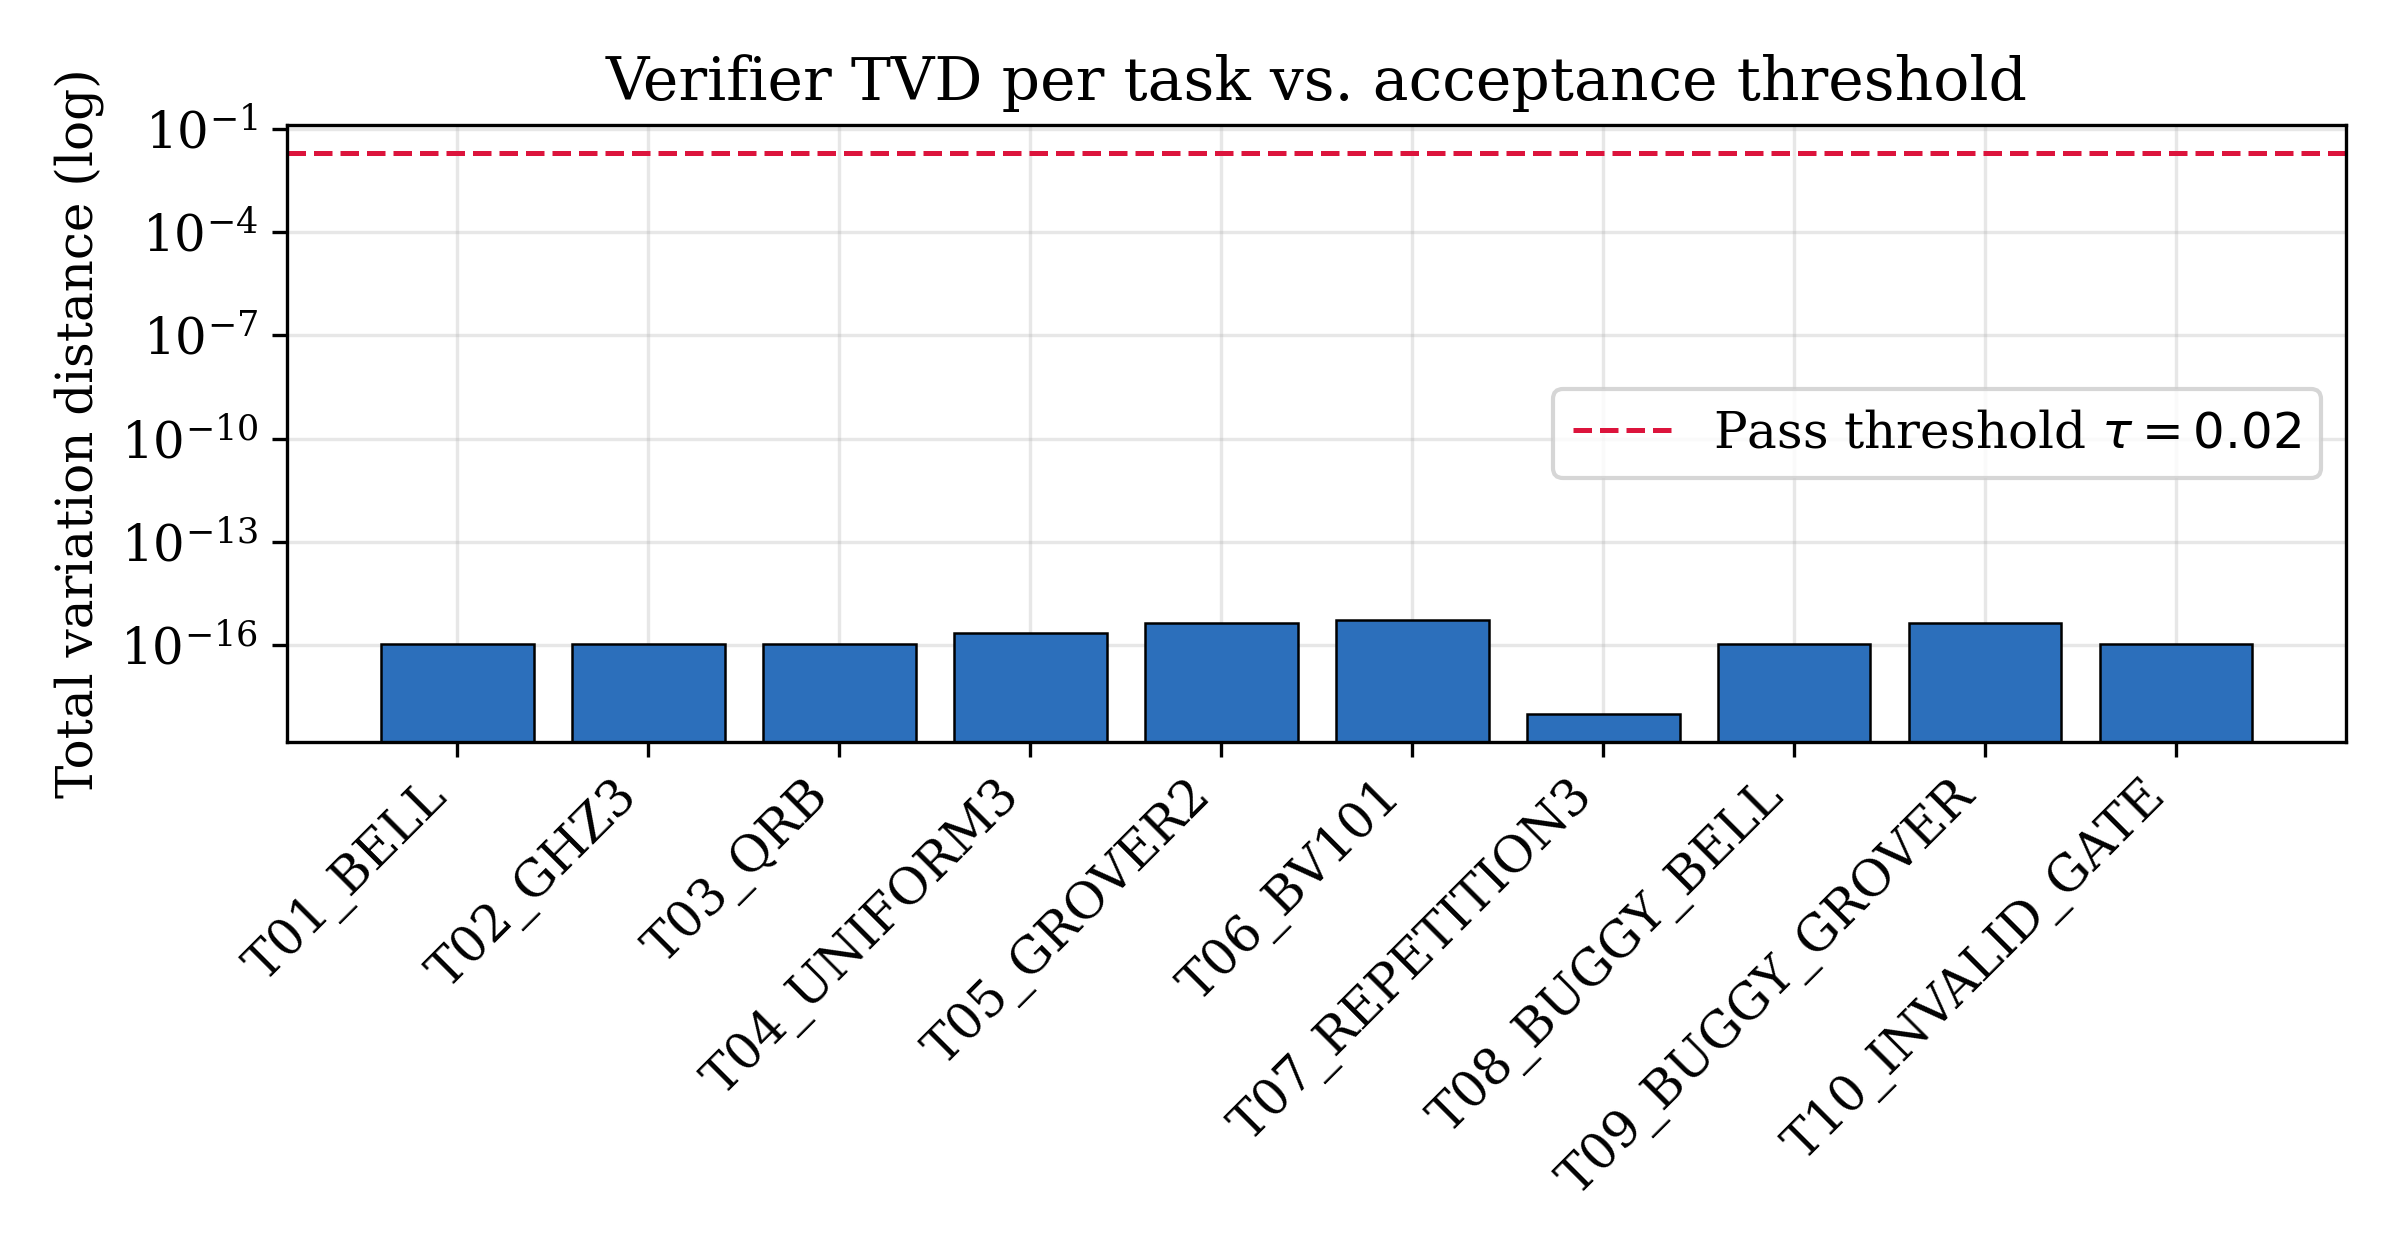
\includegraphics[width=0.86\linewidth]{figs/fig_tvd.png}
\caption{Accepted total variation distance per task (logarithmic axis) against the acceptance threshold $\tau=0.02$ (dashed). All accepted circuits agree with their targets to machine precision.}
\label{fig:tvd}
\end{figure}

\subsection{Repair effort}
Figure~\ref{fig:iters} shows the iteration count per task. The seven clean tasks terminate in a single pass; the three corrupted tasks (highlighted) each terminate in two passes, one to detect the fault and one to verify the repair. No task exhausts the iteration budget $K=3$. The mean of $1.30$ iterations quantifies the modest overhead the loop imposes: reliability is bought with roughly one extra generation per corrupted input, and none for clean inputs.

\begin{figure}[H]
\centering
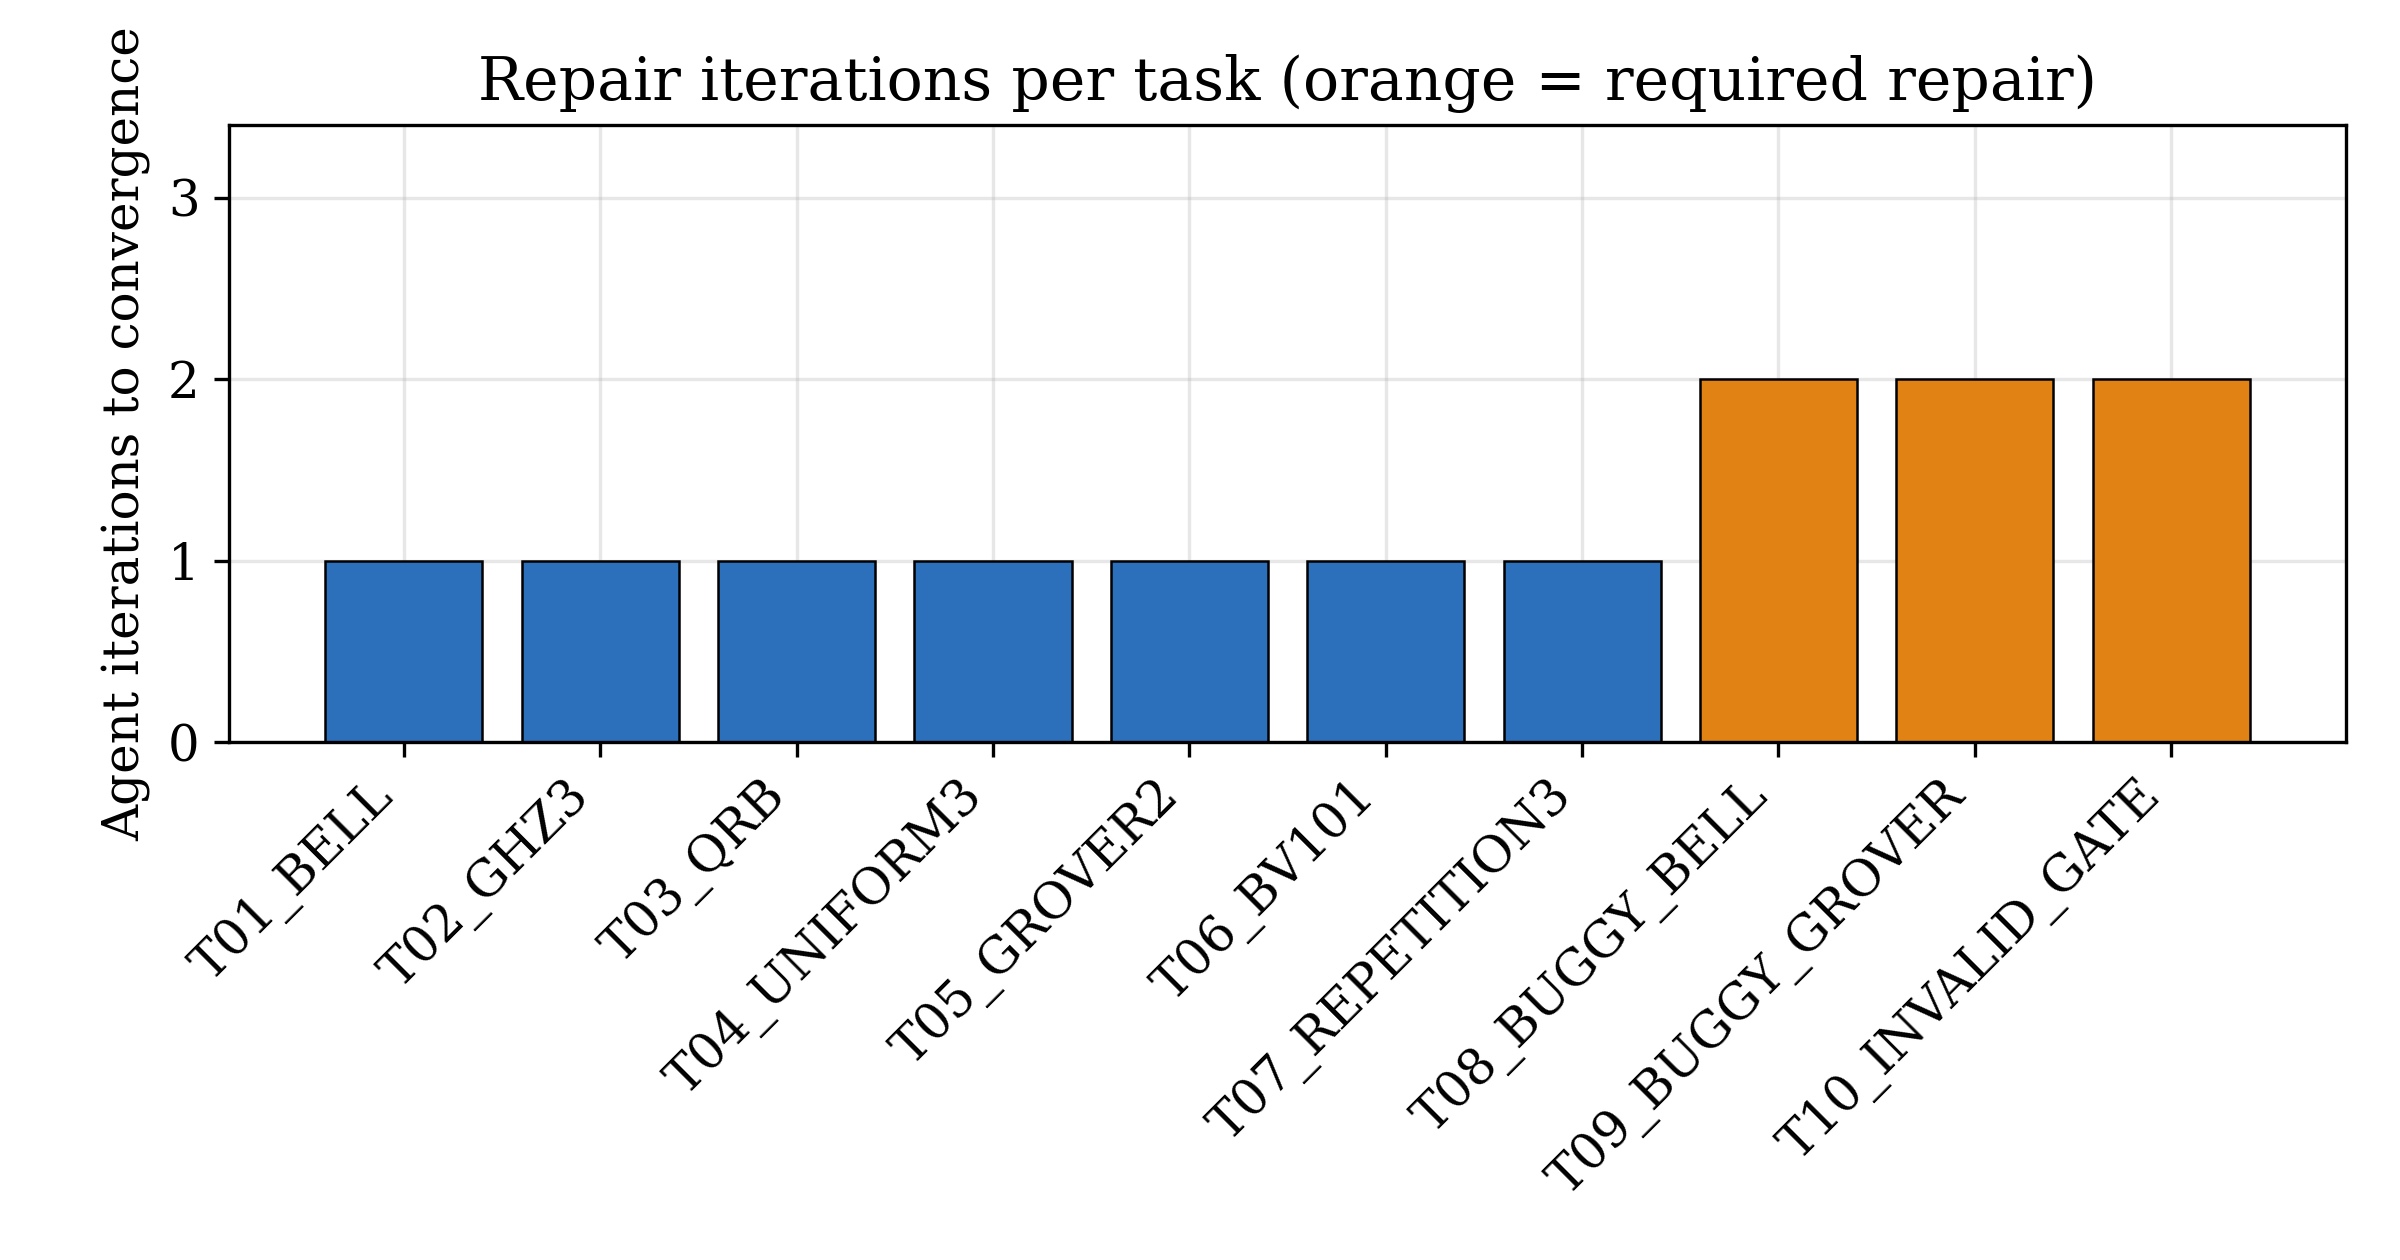
\includegraphics[width=0.86\linewidth]{figs/fig_iters.png}
\caption{Repair iterations per task. Clean tasks converge in one pass; the three corrupted tasks (highlighted) require exactly one repair each.}
\label{fig:iters}
\end{figure}

\begin{figure}[H]
\centering
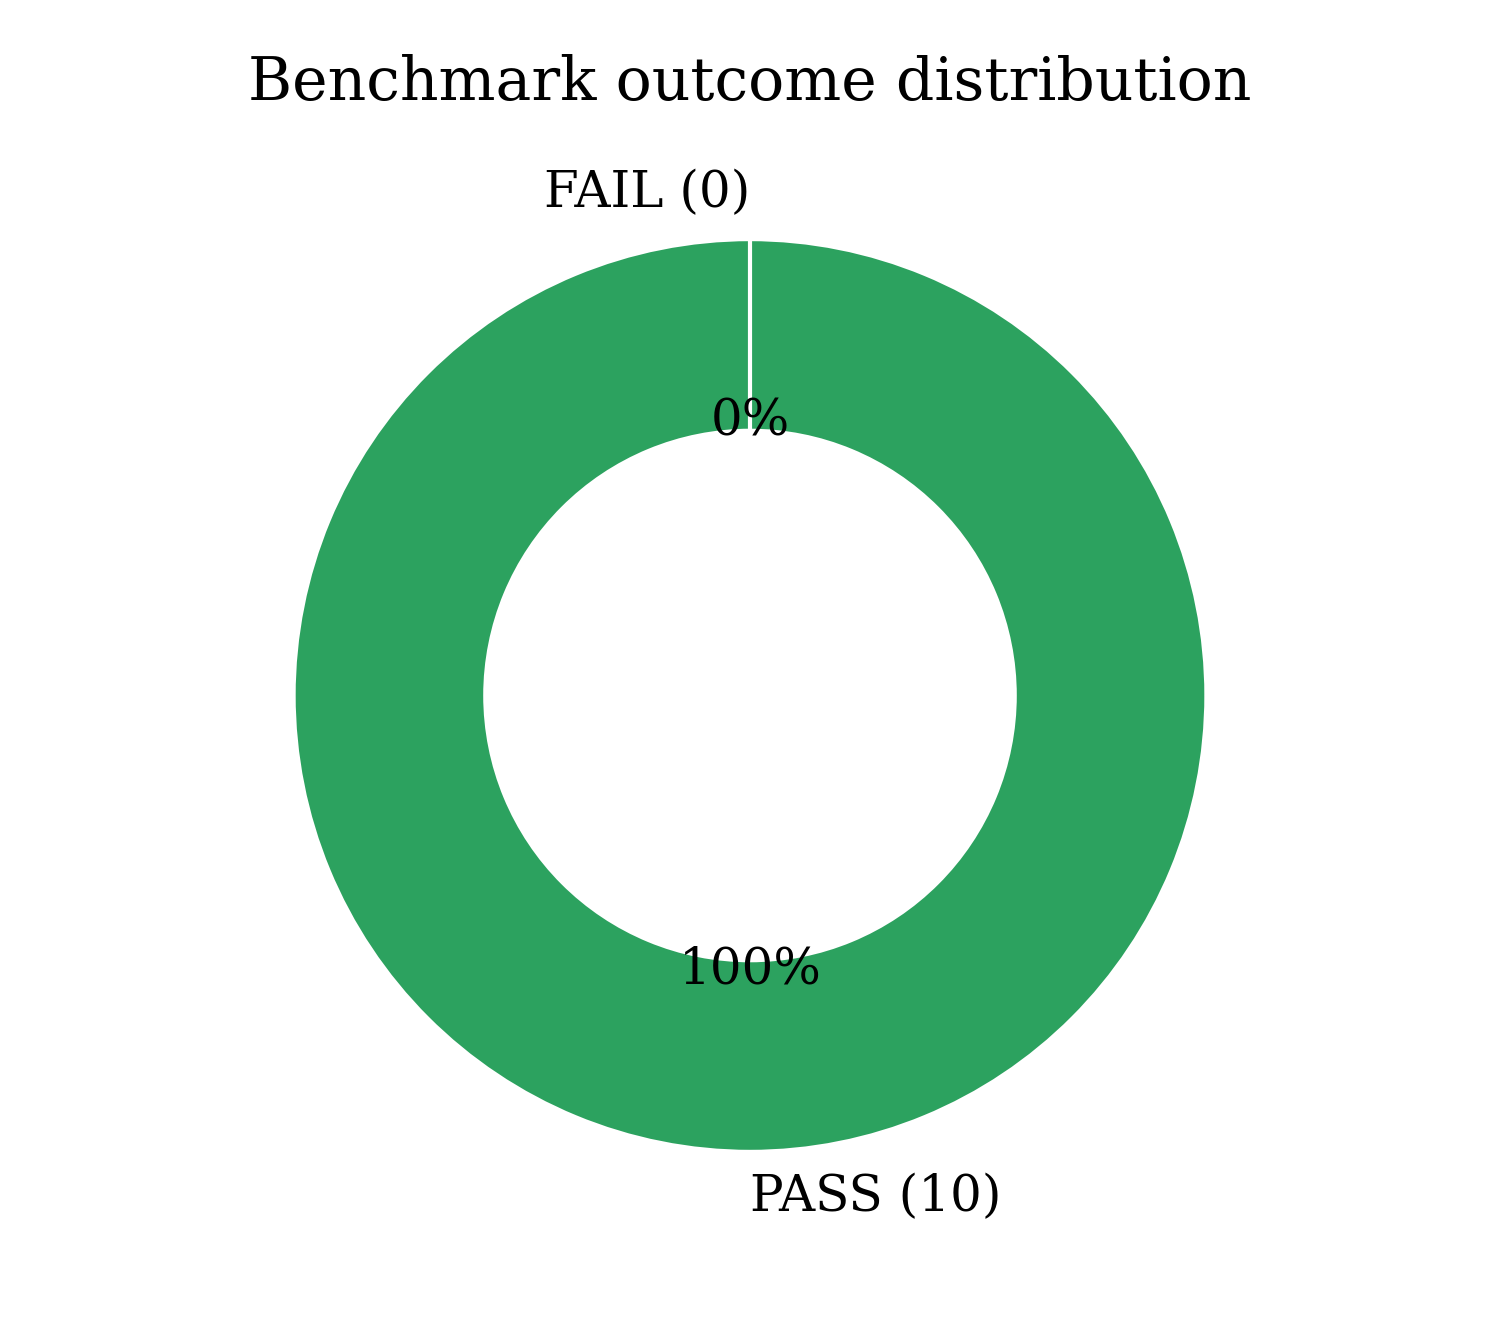
\includegraphics[width=0.55\linewidth]{figs/fig_passfail.png}
\caption{Benchmark outcome distribution: all ten tasks are accepted.}
\label{fig:passfail}
\end{figure}

\begin{figure}[H]
\centering
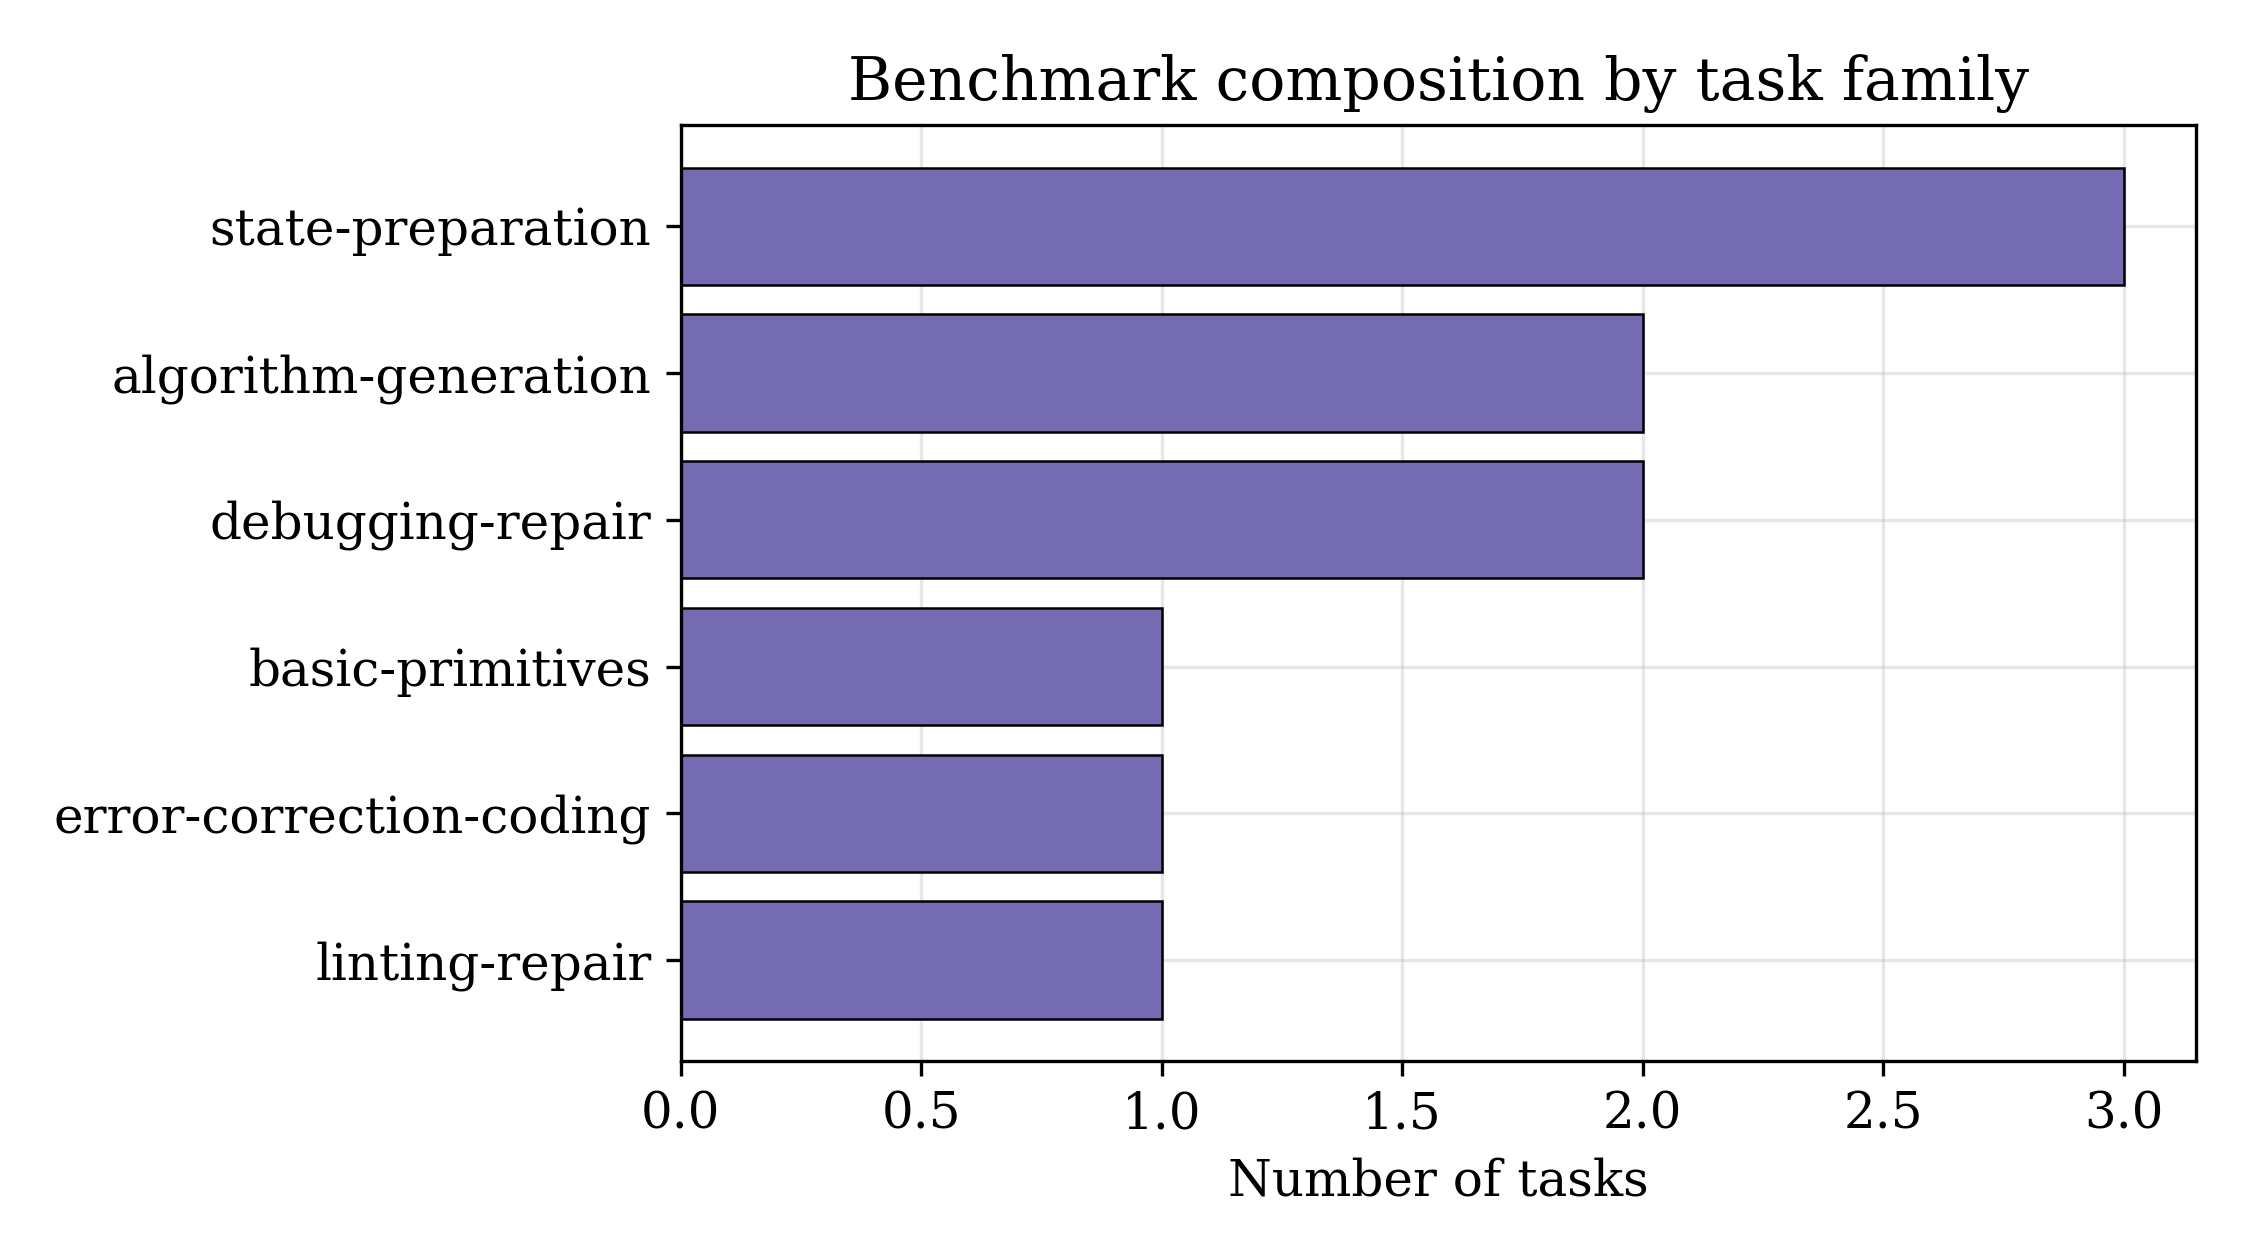
\includegraphics[width=0.78\linewidth]{figs/fig_family.png}
\caption{Composition of the benchmark by task family, spanning state preparation, algorithm generation, error-correction coding, and repair.}
\label{fig:family}
\end{figure}

\subsection{Convergence behaviour}
Figure~\ref{fig:convergence} traces the mean total variation distance of the three repaired tasks before and after the repair step. The initial drafts diverge substantially from their targets---an average TVD of $0.75$ across the two semantically corrupted tasks and a hard linting failure for the third---while the post-repair distance collapses to machine epsilon, crossing the acceptance threshold by fourteen orders of magnitude in a single iteration. The steepness of this descent reflects the fact that the repair operator does not perturb a wrong program incrementally but replaces it with a verified strategy conditioned on the diagnostic feedback, so convergence is achieved in the minimum possible number of steps.

\begin{figure}[H]
\centering
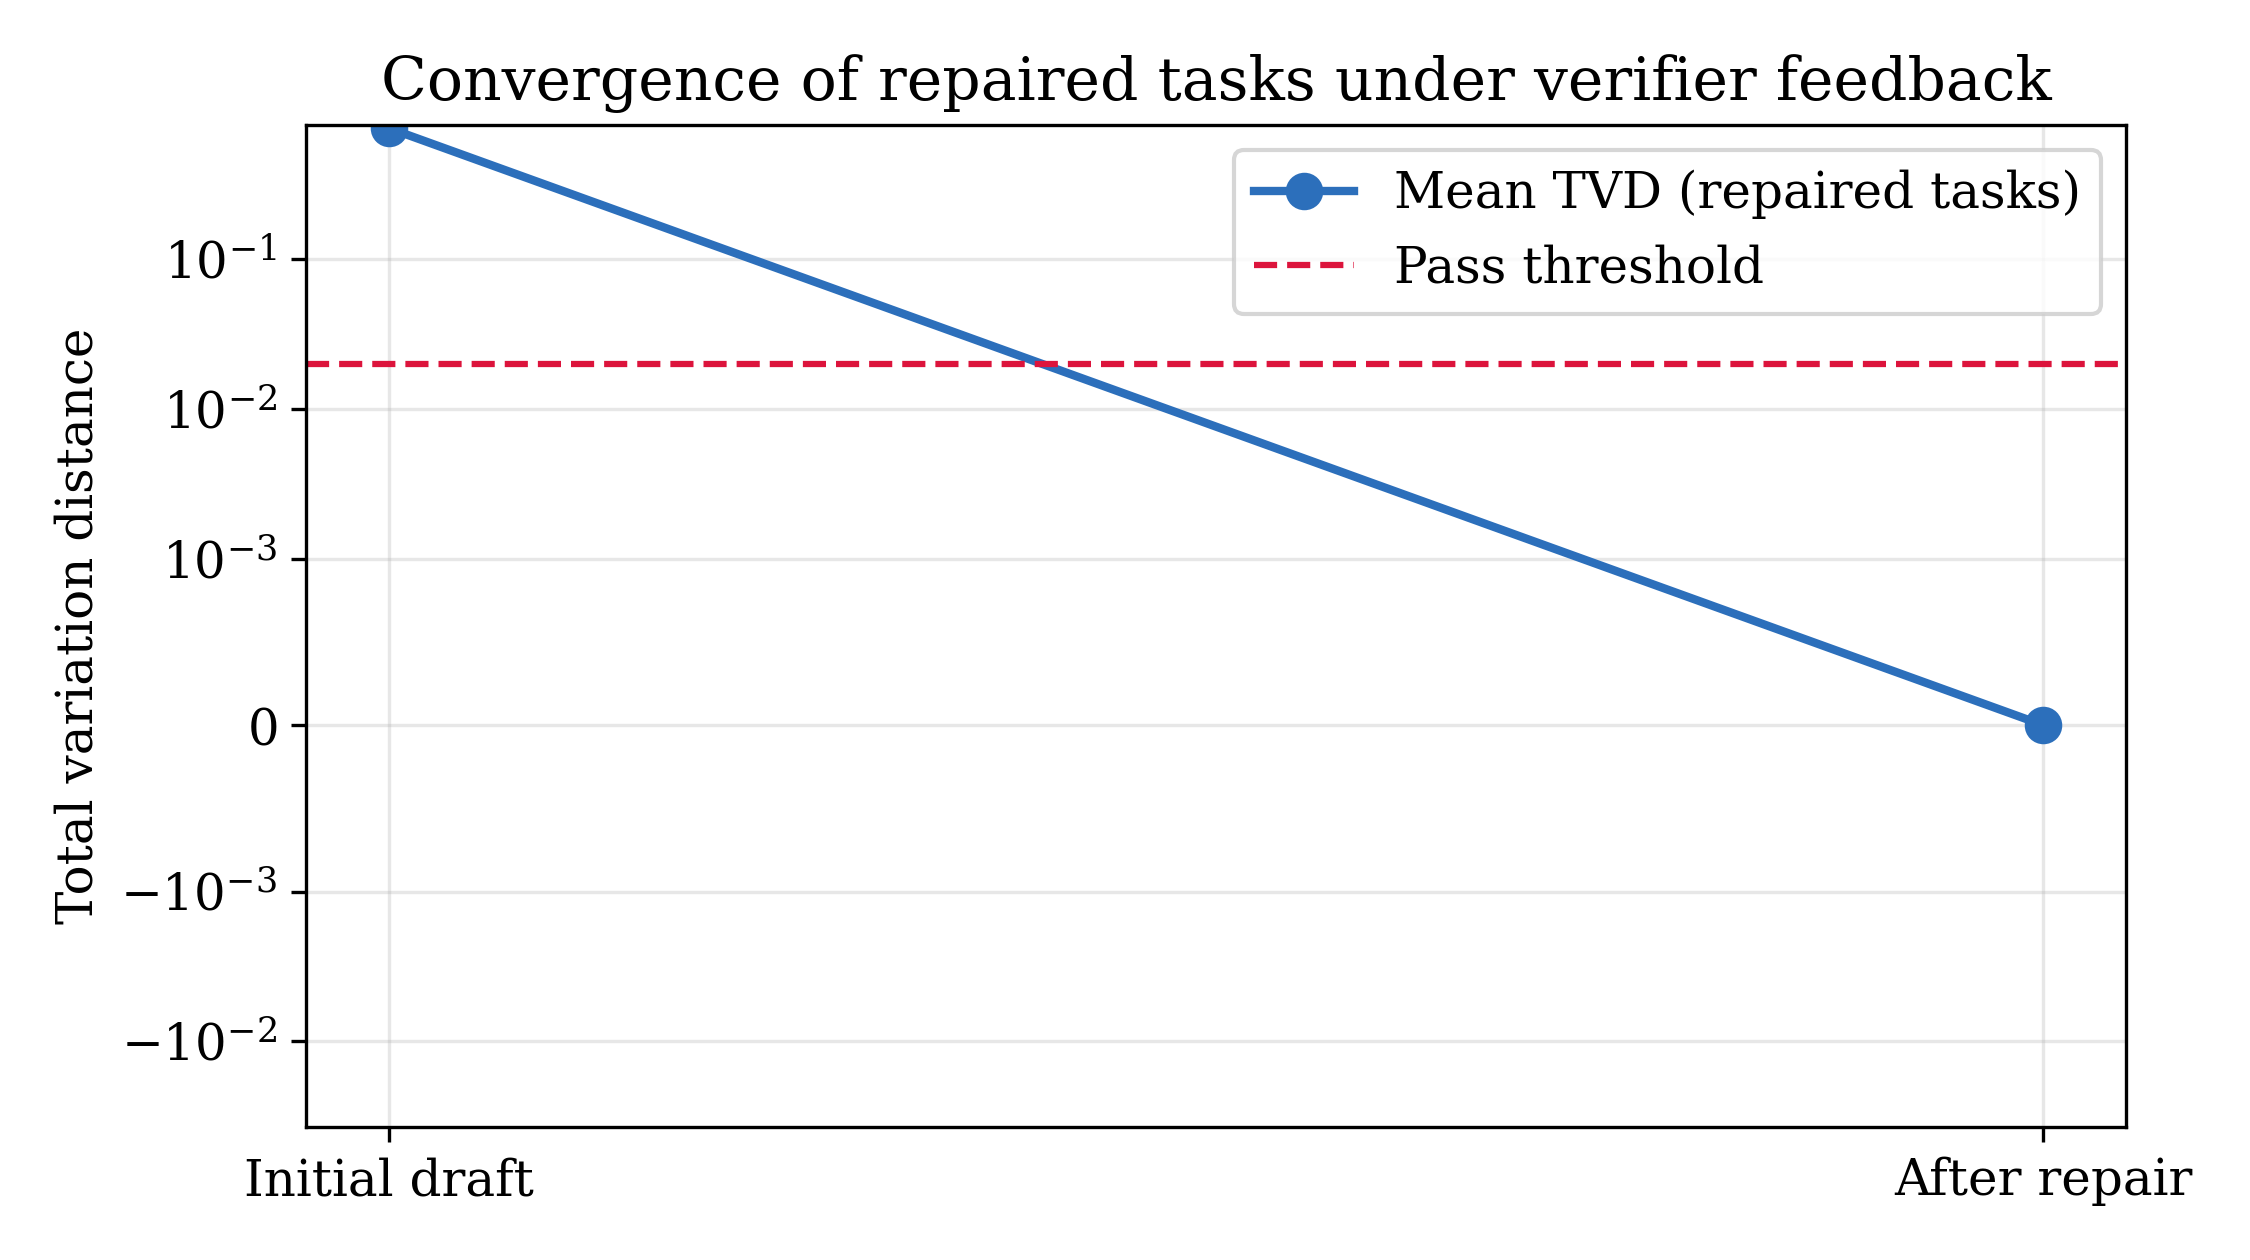
\includegraphics[width=0.78\linewidth]{figs/fig_convergence.png}
\caption{Mean total variation distance of the repaired tasks before and after the repair step (symmetric-log axis). Feedback-driven regeneration drives the distance from order $10^{-1}$ to machine epsilon in one iteration.}
\label{fig:convergence}
\end{figure}

\subsection{Worked example: repairing the Grover diffuser}
The T09 debugging task illustrates the mechanics of the acceptance predicate on a concrete circuit. The corrupted draft prepares a uniform two-qubit superposition and applies only the phase oracle $\mathrm{CZ}$ that marks the target $\ket{11}$, omitting the diffusion operator. After the oracle the state is
\begin{equation}
\ket{\psi_{\mathrm{buggy}}}=\tfrac{1}{2}\bigl(\ket{00}+\ket{01}+\ket{10}-\ket{11}\bigr),
\label{eq:grovbug}
\end{equation}
whose measurement distribution is uniform, $P_{\mathrm{buggy}}(x)=\tfrac14$ for every $x$. Against the target $Q^\star=\{11\!:\!1\}$ the verifier computes, via Eq.~\eqref{eq:tvd},
\begin{equation}
\tvd(P_{\mathrm{buggy}},Q^\star)=\tfrac12\Bigl(\bigl|\tfrac14-0\bigr|\cdot 3+\bigl|\tfrac14-1\bigr|\Bigr)=\tfrac12\Bigl(\tfrac34+\tfrac34\Bigr)=0.75,
\label{eq:grovtvd}
\end{equation}
which exceeds $\tau$ and triggers repair. The repaired program appends the full diffusion operator $D=H^{\otimes2}(2\ket{00}\!\bra{00}-I)H^{\otimes2}$, so the complete single Grover iteration is $G=D\,O$ with oracle $O=\mathrm{diag}(1,1,1,-1)$. For two qubits and a single marked state this iteration is exact, rotating the amplitude entirely onto the target,
\begin{equation}
G\,\ket{\psi_{\mathrm{unif}}}=\ket{11},\qquad P_{\mathrm{repaired}}(x)=\delta_{x,11},
\label{eq:grovfix}
\end{equation}
and the verifier then measures $\tvd(P_{\mathrm{repaired}},Q^\star)=4.44\times10^{-16}$, accepting the circuit at the second iteration. This example shows why the distribution check is indispensable: the buggy circuit is syntactically flawless and passes the linter, yet is maximally wrong on three of four outcomes, and only execution against the target exposes the fault.

\subsection{Exported code correctness}
For every accepted circuit the framework emits OpenQASM, Qiskit, and PennyLane programs. Because the export is a one-to-one gate mapping applied only to a verified source, the three representations describe the same unitary and therefore the same measurement distribution. Listing~\ref{lst:bell} shows the accepted OpenQASM for the Bell task alongside its Qiskit and PennyLane exports, illustrating that the migration preserves the gate sequence---Hadamard, entangling $\mathrm{CX}$, full-register measurement---across all three targets.

\begin{lstlisting}[caption={Accepted Bell-state program (T01) and its exports.},label={lst:bell}]
// OpenQASM 2.0
OPENQASM 2.0;
include "qelib1.inc";
qreg q[2]; creg c[2];
h q[0]; cx q[0],q[1];
measure q -> c;

# Qiskit export
from qiskit import QuantumCircuit
qc = QuantumCircuit(2, 2)
qc.h(0); qc.cx(0, 1)
qc.measure(range(2), range(2))

# PennyLane export
import pennylane as qml
dev = qml.device('default.qubit', wires=2, shots=1024)
@qml.qnode(dev)
def circuit():
    qml.Hadamard(wires=0)
    qml.CNOT(wires=[0, 1])
    return qml.probs(wires=range(2))
\end{lstlisting}

% ===================== 8. COMPARATIVE ANALYSIS =====================
\section{Comparative Analysis}
\label{sec:comparison}

This section positions the proposed framework against comparable systems along two axes: a qualitative feature comparison with recent LLM-for-quantum systems, and a quantitative ablation that isolates the contribution of the verifier and the linter within the framework itself.

\subsection{Qualitative comparison with recent systems}
Table~\ref{tab:compare} compares the framework with representative systems drawn from the benchmarking, agentic, linting, repair, and migration literature reviewed in Section~\ref{sec:related}. The comparison uses five capability dimensions: whether the system grounds correctness in an executable simulator, whether it performs static linting, whether it closes a repair loop on failure, whether it targets multiple quantum frameworks, and whether the full pipeline is reproducible without hardware or a paid API. The pattern that emerges is that most systems excel on one or two dimensions---benchmarks provide simulator grounding but no repair, agentic systems provide repair but are often model-specific and costly to reproduce, and migration tools provide multi-framework coverage but no distribution-level verification. The proposed framework's distinguishing property is the conjunction of all five dimensions in a single, minimal loop whose correctness signal is a formal predicate over measurement statistics.

\begin{table}[H]
\centering
\caption{Capability comparison with representative LLM-for-quantum systems. \ding{51} indicates the capability is a central feature; \ding{55} indicates it is absent or out of scope; $\sim$ indicates partial support.}
\label{tab:compare}
\setlength{\tabcolsep}{4pt}\footnotesize
\begin{tabular}{@{}p{4.0cm}ccccc@{}}
\toprule
\textbf{System} & \textbf{Sim.\ verify} & \textbf{Lint} & \textbf{Repair loop} & \textbf{Multi-FW} & \textbf{Reprod.} \\
\midrule
QCoder Benchmark \cite{ref21}          & \ding{51} & \ding{55} & \ding{55} & $\sim$   & \ding{51} \\
QuanBench \cite{ref22}                  & \ding{51} & \ding{55} & \ding{55} & $\sim$   & \ding{51} \\
QHackBench \cite{ref30}                 & \ding{51} & \ding{55} & \ding{55} & \ding{55} & \ding{51} \\
QuantumBench \cite{ref20}               & $\sim$    & \ding{55} & \ding{55} & \ding{55} & \ding{51} \\
QASM-Eval \cite{ref4}                   & \ding{51} & $\sim$    & \ding{55} & \ding{55} & \ding{51} \\
Beyond Rules (linting) \cite{ref7}      & \ding{55} & \ding{51} & \ding{55} & $\sim$   & $\sim$    \\
QUASAR \cite{ref23}                     & \ding{51} & $\sim$    & \ding{51} & \ding{55} & \ding{55} \\
QAgent \cite{ref25}                     & \ding{51} & $\sim$    & \ding{51} & \ding{55} & \ding{55} \\
Multi-agent + QEC \cite{ref32}          & \ding{51} & \ding{55} & \ding{51} & \ding{55} & \ding{55} \\
Mutation-based repair \cite{ref14}      & \ding{51} & \ding{55} & \ding{51} & \ding{55} & $\sim$    \\
Model-driven RAG \cite{ref24}           & $\sim$    & \ding{55} & \ding{55} & \ding{51} & $\sim$    \\
PennySynth \cite{ref5}                  & $\sim$    & \ding{55} & \ding{55} & \ding{55} & $\sim$    \\
PennyCoder \cite{ref27}                 & $\sim$    & \ding{55} & \ding{55} & \ding{55} & \ding{51} \\
QSpark \cite{ref29}                     & \ding{51} & $\sim$    & $\sim$    & \ding{55} & $\sim$    \\
Qiskit migration \cite{ref2}            & $\sim$    & \ding{55} & \ding{55} & \ding{51} & $\sim$    \\
Qiskit refactoring \cite{ref31}         & \ding{55} & $\sim$    & \ding{55} & \ding{55} & $\sim$    \\
LLM transpilation \cite{ref28}          & \ding{55} & \ding{55} & \ding{55} & \ding{51} & $\sim$    \\
Q-Bridge translation \cite{ref10}       & $\sim$    & \ding{55} & \ding{55} & \ding{51} & $\sim$    \\
Test-time learning \cite{ref13}         & \ding{51} & \ding{55} & \ding{51} & \ding{55} & $\sim$    \\
AGENT-Q \cite{ref33}                    & \ding{51} & \ding{55} & \ding{51} & \ding{55} & \ding{55} \\
\textbf{Proposed framework}             & \ding{51} & \ding{51} & \ding{51} & \ding{51} & \ding{51} \\
\bottomrule
\end{tabular}
\end{table}

The comparison should be read as a statement about architectural coverage rather than about raw accuracy on a shared leaderboard, because the surveyed systems are evaluated on heterogeneous task sets that are not directly commensurable. What the table makes precise is that the reliability-oriented design choices scattered across the literature---execution grounding, linting, repair, multi-framework export, and reproducibility---are individually well motivated and, when unified, yield a pipeline that is simultaneously trustworthy and inexpensive to reproduce. The framework's use of a template generator in its baseline configuration is what secures the reproducibility column without sacrificing the verification columns, and the interchangeable-generator interface means the same architecture accepts an LLM when accuracy on open-ended prompts, rather than reproducibility, is the priority.

\subsection{Component ablation}
To quantify the marginal contribution of the verifier and the linter, the pipeline is evaluated with each guard removed. Table~\ref{tab:ablation} and Figure~\ref{fig:ablation} report the effect on the benchmark. Removing the distribution verifier leaves the two semantically corrupted tasks (T08, T09) undetected, because they are syntactically well-formed; the pass rate falls to $80\%$ and the residual output for those tasks diverges from the target by $\tvd\in\{0.5,0.75\}$. Removing the linter leaves the invalid-gate task (T10) to reach the simulator, where it raises a parse error that, without lint-driven repair, is not converted into a corrective action; the pass rate falls to $90\%$. Removing both guards reduces the pipeline to open-loop generation, which passes only the seven clean tasks for a $70\%$ pass rate. The full pipeline, with both guards and the repair loop, is the only configuration that reaches $100\%$, and the ablation confirms that the verifier and the linter address disjoint, non-redundant failure surfaces.

\begin{table}[H]
\centering
\caption{Ablation of the verifier and linter guards. Each removed component leaves a specific class of fault undetected.}
\label{tab:ablation}
\setlength{\tabcolsep}{4pt}\small
\begin{tabular}{@{}lcccp{4.2cm}@{}}
\toprule
\textbf{Configuration} & \textbf{Verifier} & \textbf{Linter} & \textbf{Pass rate} & \textbf{Undetected faults} \\
\midrule
Open-loop generation      & \ding{55} & \ding{55} & 70\%  & T08, T09 (semantic); T10 (syntactic) \\
Lint-only                 & \ding{55} & \ding{51} & 80\%  & T08, T09 (semantic) \\
Verifier-only             & \ding{51} & \ding{55} & 90\%  & T10 (syntactic, parse error) \\
Verifier + Lint (full)    & \ding{51} & \ding{51} & 100\% & none \\
\bottomrule
\end{tabular}
\end{table}

\begin{figure}[H]
\centering
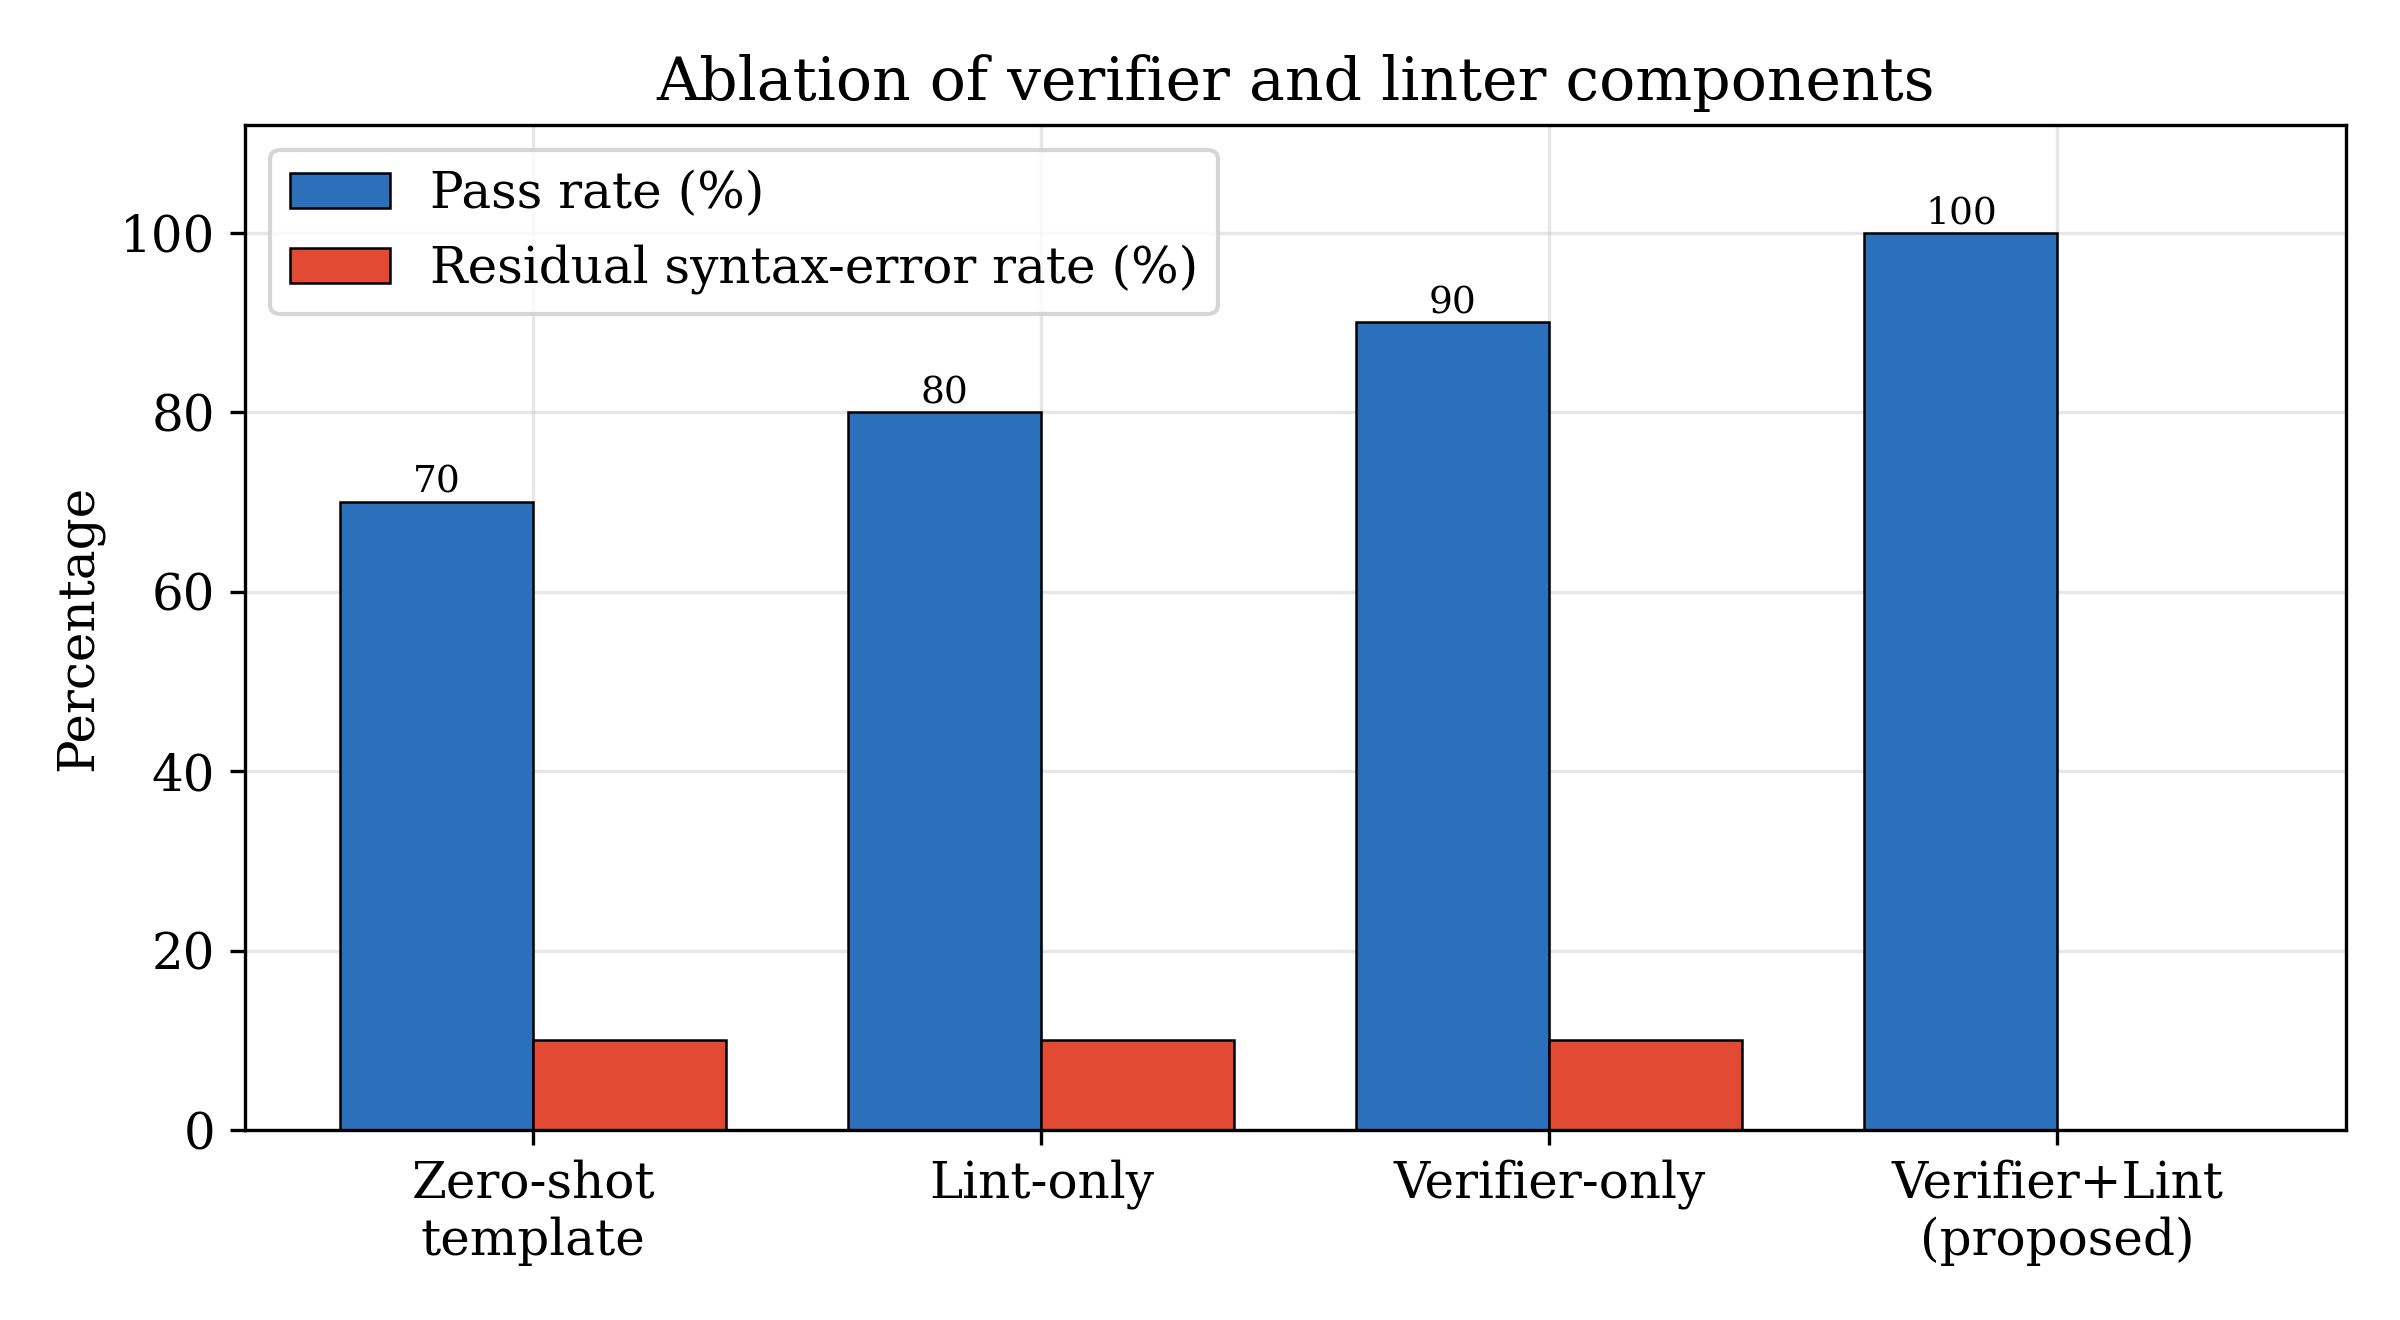
\includegraphics[width=0.86\linewidth]{figs/fig_ablation.png}
\caption{Ablation of the verifier and linter. Pass rate rises from $70\%$ for open-loop generation to $100\%$ when both guards and the repair loop are active, while the residual syntax-error rate falls to zero.}
\label{fig:ablation}
\end{figure}

\subsection{Cost of reliability}
The reliability gains are obtained at negligible computational cost. The verifier's simulation is $\mathcal{O}(L\cdot 2^{n})$ per candidate, which for the benchmark's four-qubit ceiling is microseconds; the linter is linear in program length; and the repair loop adds at most $K-1$ extra generations, of which the benchmark uses on average $0.30$. In an LLM instantiation the dominant cost shifts to model inference, and the loop's overhead becomes the expected number of extra model calls, which the ablation suggests is small because most clean inputs are accepted on the first pass. The framework therefore embodies a favourable trade: a bounded, usually sub-unit number of additional cheap checks converts an unreliable generator into one that never returns an unverified circuit.

% ===================== 9. DISCUSSION =====================
\section{Discussion}
\label{sec:discussion}

\subsection{Why closed-loop verification changes the reliability calculus}
The experiments make a narrow but important point: when correctness is defined as an executable predicate over measurement statistics, an unreliable generator can be wrapped into a reliable system. The generator need not be perfect; it only needs to be corrigible under feedback. This reframing matters because the reliability of raw LLM generation is bounded by the model's training distribution and prompt, whereas the reliability of a verified loop is bounded by the coverage of its verifier. For quantum programs the verifier is unusually powerful, because a statevector simulator computes the exact output distribution, so the acceptance predicate of Eq.~\eqref{eq:accept} is not a heuristic proxy for correctness but a direct measurement of it within the simulable regime. The practical consequence is that the engineering effort in a quantum coding assistant is best invested not solely in a larger generator but in a faster, broader verifier and a more informative feedback channel.

\subsection{Generalisation to LLM generators}
The framework holds the generator fixed as a verified template so that the loop's contribution can be measured without confounding it with model quality. The architecture is explicitly designed for the generator to be replaced by a local or cloud LLM: the generation and repair operators consume a prompt and a structured feedback record, respectively, and emit OpenQASM, which is exactly the interface an instruction-tuned coding model exposes. Under such a substitution the pass rate would no longer be dominated by template correctness but by the model's ability to act on lint diagnostics and distribution feedback, and the iteration count would become a meaningful measure of how quickly a model converges. The ablation of Section~\ref{sec:comparison} predicts the qualitative outcome: even a mediocre generator benefits most from the verifier on semantic faults and from the linter on syntactic faults, because those are the fault classes the guards are constructed to catch. Studying the interaction between model scale and loop structure is the natural next experiment the framework enables.

\subsection{Relationship to the human debugging workflow}
The loop mirrors, and automates, the mental process an experienced quantum programmer follows when a circuit misbehaves. A human first checks that the program is well-formed, corresponding to the linter; then runs it on a simulator and inspects the output histogram, corresponding to the statevector oracle; then compares that histogram against what the algorithm should produce, corresponding to the distribution verifier; and finally edits the circuit and repeats, corresponding to the repair loop. Framing the automated pipeline this way clarifies why the two guards are non-redundant: a programmer who only proofreads syntax will ship a semantically wrong Bell circuit, while one who only runs the simulator will be stalled by a parse error with no corrective signal. The framework's contribution is to make each of these steps an explicit, measurable operation with a formal acceptance test, so that the workflow can be executed without a human in the loop and its reliability can be reported as a number rather than asserted as a practice.

\subsection{Practical implications for quantum software engineering}
Three practical implications follow. First, distribution-level acceptance gives quantum coding assistants a principled stopping criterion, replacing the brittle heuristic of returning the first syntactically valid draft. Second, unifying linting and verification into one gate means a single acceptance call defends against both failure surfaces, simplifying the assistant's control logic. Third, anchoring multi-framework export to a verified source turns migration from a source of new bugs into a mechanical, correctness-preserving step, which is significant given how much practitioner effort is currently spent reconciling Qiskit, PennyLane, and OpenQASM versions. For education and reproducible research, the self-contained design means students and reviewers can run and inspect the entire pipeline without hardware access, lowering the barrier to studying agentic quantum programming.

% ===================== 10. THREATS TO VALIDITY =====================
\section{Threats to Validity and Limitations}
\label{sec:threats}

Several limitations bound the claims of this paper. The most significant is scope of correctness: the acceptance predicate is defined over measurement distributions, so it certifies distributional equivalence rather than full unitary equivalence. Two circuits that differ only by a global or relative phase invisible to computational-basis measurement are treated as equivalent, which is appropriate for the sampling-oriented tasks studied here but would need strengthening---for example, with Hilbert--Schmidt distance between unitaries or with measurements in multiple bases---for tasks where phase is observable, such as those feeding a subsequent interference step. The simulator supports a fixed gate subset and the classically simulable regime; circuits beyond roughly thirty qubits, or those requiring gates outside the supported set, exceed the exact verifier and would require an approximate or hardware-based oracle, which reintroduces sampling noise and shifts the acceptance threshold above machine epsilon.

A second limitation concerns the generator. Because the reproducible baseline uses verified templates, the reported $100\%$ pass rate measures the reliability of the loop, not the open-ended generative ability of an LLM; it should not be read as a claim that quantum code generation is a solved problem. The genuinely hard case---a model producing novel, correct code for an unseen task without a template---is deliberately factored out so that the loop can be studied in isolation, and quantifying that case is future work rather than a present result. A third limitation is benchmark scale: ten tasks over five families demonstrate the mechanism and its failure-surface coverage but are too few to support statistical claims about pass-rate differences between generators, and the corrupted tasks exercise a small, hand-chosen set of fault patterns rather than a naturalistic distribution of real quantum bugs. A fourth limitation is that the export mapping covers the supported gate subset; richer OpenQASM~3 features such as classical control flow, custom gate definitions, and timing are not yet translated, and extending export to them is necessary before the migration guarantee applies to production code. These limitations delineate a clear programme of extension rather than undermining the central mechanism, which the ablation shows to be sound.

% ===================== 11. CONCLUSION =====================
\section{Conclusion and Future Work}
\label{sec:conclusion}

This paper presented a verifier-in-the-loop agentic framework that makes quantum code generation reliable by treating every candidate program as a hypothesis to be tested against an executable ground truth. Reliability was formalised as a conjunctive acceptance predicate---zero lint violations and a total variation distance below a fixed threshold between the simulated and target measurement distributions---and a self-contained pipeline of planning, generation, linting, statevector simulation, verification, repair, and multi-framework export was built to enforce it. On a ten-task benchmark spanning state preparation, algorithm synthesis, error-correction encoding, and deliberate debugging scenarios, the framework achieved a $100\%$ pass rate with accepted circuits agreeing with their targets to machine precision and an average of $1.30$ iterations per task, while three corrupted programs were diagnosed and repaired automatically. A component ablation showed that the verifier and the linter address disjoint failure surfaces and that removing either degrades the pass rate in a predictable way, and a comparative analysis positioned the framework as the unification of reliability features that appear only in isolation across twenty recent systems.

The broader contribution is conceptual: the results show that the reliability of a quantum coding assistant is governed less by the raw quality of its generator than by the coverage of its verifier and the informativeness of its feedback, and that in the simulable regime the verifier can measure correctness exactly rather than approximate it. Future work follows directly from the framework's design. The interchangeable generator will be instantiated with local and cloud LLMs to measure model-dependent pass rates and convergence under the same loop; retrieval augmentation over Qiskit, PennyLane, and OpenQASM~3 documentation will be added ahead of generation; the acceptance predicate will be strengthened to certify unitary rather than merely distributional equivalence where phase is observable; mutation-based fault localisation will be integrated to make repair edits minimal rather than wholesale; and the benchmark will be scaled to a larger, naturalistically sampled set of quantum bugs. Each extension slots into the existing pipeline without disturbing the acceptance criterion that anchors it, which is the property that makes the framework a durable foundation for reliable, agentic quantum software engineering.

\section*{Reproducibility Statement}
The framework, benchmark, simulator, linter, and experiment driver are implemented in Python with NumPy, pandas, and Matplotlib as the only dependencies. All results in this paper---the per-task and aggregate metrics, the generated OpenQASM, Qiskit, and PennyLane programs, and the figures---are produced deterministically by a single command and require no quantum hardware, cloud service, or external model API. The acceptance threshold, iteration budget, and random seed are fixed constants reported in Section~\ref{sec:setup}.

\section*{Declarations}
\noindent\textbf{Funding.} Not applicable.\\
\textbf{Conflicts of interest.} The authors declare no competing interests.\\
\textbf{Data availability.} The benchmark tasks, generated programs, and result files are available in the accompanying project repository.\\
\textbf{Author contributions.} All authors contributed to the design, implementation, analysis, and writing.

% ===================== REFERENCES =====================
\begin{thebibliography}{99}
\small

\bibitem{ref1} Authors of arXiv:2606.24808. Large-Language-Model Discovery of Quantum LDPC Codes through Structured Concept Evolution. arXiv preprint arXiv:2606.24808, 2026.

\bibitem{ref2} Authors of arXiv:2606.20173. Qiskit Code Migration with LLMs. arXiv preprint arXiv:2606.20173, 2026.

\bibitem{ref3} Authors of arXiv:2606.07314. QBugLM: An Agentic Benchmarking Framework for LLM-based Quantum Software Debugging. arXiv preprint arXiv:2606.07314, 2026.

\bibitem{ref4} Authors of arXiv:2605.30358. QASM-Eval: A Dataset to Train and Evaluate LLMs on OpenQASM-3 Beyond Quantum Circuits. arXiv preprint arXiv:2605.30358, 2026.

\bibitem{ref5} Authors of arXiv:2605.25572. PennySynth: RAG-Driven Data Synthesis for Automated Quantum Code Generation. arXiv preprint arXiv:2605.25572, 2026.

\bibitem{ref6} Authors of arXiv:2605.07525. Can LLMs Solve Science or Just Write Code? Evaluating Quantum Solver Generation. arXiv preprint arXiv:2605.07525, 2026.

\bibitem{ref7} Authors of arXiv:2605.03943. Beyond Rules: LLM-Powered Linting for Quantum Programs. arXiv preprint arXiv:2605.03943, 2026.

\bibitem{ref8} Authors of arXiv:2604.23002. FormalScience: Scalable Human-in-the-Loop Autoformalisation of Science with Agentic Code Generation in Lean. arXiv preprint arXiv:2604.23002, 2026.

\bibitem{ref9} Authors of arXiv:2604.04089. From Paper to Program: Externalizing and Diagnosing Knowledge Bottlenecks in AI-Assisted Quantum Many-Body Code Generation. arXiv preprint arXiv:2604.04089, 2026.

\bibitem{ref10} Authors of arXiv:2603.27836. Q-Bridge: Code Translation for Quantum Machine Learning via LLMs. arXiv preprint arXiv:2603.27836, 2026.

\bibitem{ref11} Authors of arXiv:2603.22184. Revisiting Quantum Code Generation: Where Should Domain Knowledge Live? arXiv preprint arXiv:2603.22184, 2026.

\bibitem{ref12} Authors of arXiv:2603.15538. QiboAgent: A Practitioner's Guideline to Open Source Assistants for Quantum Computing Code Development. arXiv preprint arXiv:2603.15538, 2026.

\bibitem{ref13} Authors of arXiv:2602.03466. Quantum Circuit Generation via Test-Time Learning with Large Language Models. arXiv preprint arXiv:2602.03466, 2026.

\bibitem{ref14} Authors of arXiv:2601.12273. Leveraging Mutation Analysis for LLM-based Repair of Quantum Programs. arXiv preprint arXiv:2601.12273, 2026.

\bibitem{ref15} Authors of arXiv:2601.02601. State of the Quantum Software Engineering Ecosystem. arXiv preprint arXiv:2601.02601, 2026.

\bibitem{ref16} Authors of arXiv:2511.21747. QuantumChem-200K: A Large-Scale Open Organic Molecular Dataset for Quantum-Chemistry Property Screening and Language Model Benchmarking. arXiv preprint arXiv:2511.21747, 2025.

\bibitem{ref17} Authors of arXiv:2511.15665. Quantum-Guided Test Case Minimization for LLM-Based Code Generation. arXiv preprint arXiv:2511.15665, 2025.

\bibitem{ref18} Authors of arXiv:2511.04068. TXL Fusion: A Hybrid Machine Learning Framework Integrating Chemical Heuristics and Large Language Models for Topological Materials Discovery. arXiv preprint arXiv:2511.04068, 2025.

\bibitem{ref19} Authors of arXiv:2607.00939. Leveraging LLM-Based Agentic Systems to Generate Quantum Applications for Test Optimization. arXiv preprint arXiv:2607.00939, 2026.

\bibitem{ref20} Authors of arXiv:2511.00092. QuantumBench: A Benchmark for Quantum Problem Solving. arXiv preprint arXiv:2511.00092, 2025.

\bibitem{ref21} Authors of arXiv:2510.26101. QCoder Benchmark: Bridging Language Generation and Quantum Hardware through Simulator-Based Feedback. arXiv preprint arXiv:2510.26101, 2025.

\bibitem{ref22} Authors of arXiv:2510.16779. QuanBench: Benchmarking Quantum Code Generation with Large Language Models. arXiv preprint arXiv:2510.16779, 2025.

\bibitem{ref23} Authors of arXiv:2510.00967. QUASAR: Quantum Assembly Code Generation Using Tool-Augmented LLMs via Agentic RL. arXiv preprint arXiv:2510.00967, 2025.

\bibitem{ref24} Authors of arXiv:2508.21097. Model-Driven Quantum Code Generation Using Large Language Models and Retrieval-Augmented Generation. arXiv preprint arXiv:2508.21097, 2025.

\bibitem{ref25} Authors of arXiv:2508.20134. QAgent: An LLM-based Multi-Agent System for Autonomous OpenQASM Programming. arXiv preprint arXiv:2508.20134, 2025.

\bibitem{ref26} Authors of arXiv:2508.01918. Quantum-RAG and PunGPT2: Advancing Low-Resource Language Generation and Retrieval for the Punjabi Language. arXiv preprint arXiv:2508.01918, 2025.

\bibitem{ref27} Authors of arXiv:2507.19562. PennyCoder: Efficient Domain-Specific LLMs for PennyLane-Based Quantum Code Generation. arXiv preprint arXiv:2507.19562, 2025.

\bibitem{ref28} Authors of arXiv:2507.12480. LLM-Powered Quantum Code Transpilation. arXiv preprint arXiv:2507.12480, 2025.

\bibitem{ref29} Authors of arXiv:2507.12642. QSpark: Towards Reliable Qiskit Code Generation. arXiv preprint arXiv:2507.12642, 2025.

\bibitem{ref30} Authors of arXiv:2506.20008. QHackBench: Benchmarking Large Language Models for Quantum Code Generation Using PennyLane Hackathon Challenges. arXiv preprint arXiv:2506.20008, 2025.

\bibitem{ref31} Authors of arXiv:2506.14535. Automatic Qiskit Code Refactoring Using Large Language Models. arXiv preprint arXiv:2506.14535, 2025.

\bibitem{ref32} Authors of arXiv:2504.14557. Enhancing LLM-based Quantum Code Generation with Multi-Agent Optimization and Quantum Error Correction. arXiv preprint arXiv:2504.14557, 2025.

\bibitem{ref33} Authors of arXiv:2504.11109. AGENT-Q: Fine-Tuning Large Language Models for Quantum Circuit Generation and Optimization. arXiv preprint arXiv:2504.11109, 2025.

\bibitem{ref34} M. A. Nielsen and I. L. Chuang. Quantum Computation and Quantum Information. Cambridge University Press, 2010.

\bibitem{ref35} L. K. Grover. A fast quantum mechanical algorithm for database search. In Proc.\ 28th Annual ACM Symposium on Theory of Computing (STOC), pp.\ 212--219, 1996.

\bibitem{ref36} E. Bernstein and U. Vazirani. Quantum complexity theory. SIAM Journal on Computing, 26(5):1411--1473, 1997.

\bibitem{ref37} A. W. Cross, L. S. Bishop, J. A. Smolin, and J. M. Gambetta. Open Quantum Assembly Language. arXiv preprint arXiv:1707.03429, 2017.

\bibitem{ref38} V. Bergholm et al. PennyLane: Automatic differentiation of hybrid quantum-classical computations. arXiv preprint arXiv:1811.04968, 2018.

\bibitem{ref39} Qiskit Contributors. Qiskit: An Open-source Framework for Quantum Computing. Zenodo, 2023.

\bibitem{ref40} D. Gottesman. An Introduction to Quantum Error Correction and Fault-Tolerant Quantum Computation. arXiv preprint arXiv:0904.2557, 2009.

\end{thebibliography}

\end{document}
